\Chapter{2D platformer játék tervezése és fejlesztése a Unity játékmotor segítségével}

\Section{A játék leírása}

A szakdolgozatom során szerettem volna egy 2D-s platformer játékot megalkotni. A jaték elkészítéséhez az Asset Store-ból szereztem be egy ingyenes asset-et. A játék főszereplője egy agilis, dinamikus karakter, aki a klasszikus platformer hősök hagyományait követi. A karakter alapvető mozgásai közé tartozik a futás, az ugrás és a guggolás, valamint a pályák átvihetősége érdekében bevezetésre került a grappling hook mechanika. Ezek a mozgások intuitívek és könnyen kezelhetők, miközben lehetőséget adnak a játékosoknak a pályák különböző kihívásainak megoldására. A játék vezérlőelemei \aref{fig:vezerloelemek}. ábrán láthatóak.

\begin{figure}[ht]
\centering
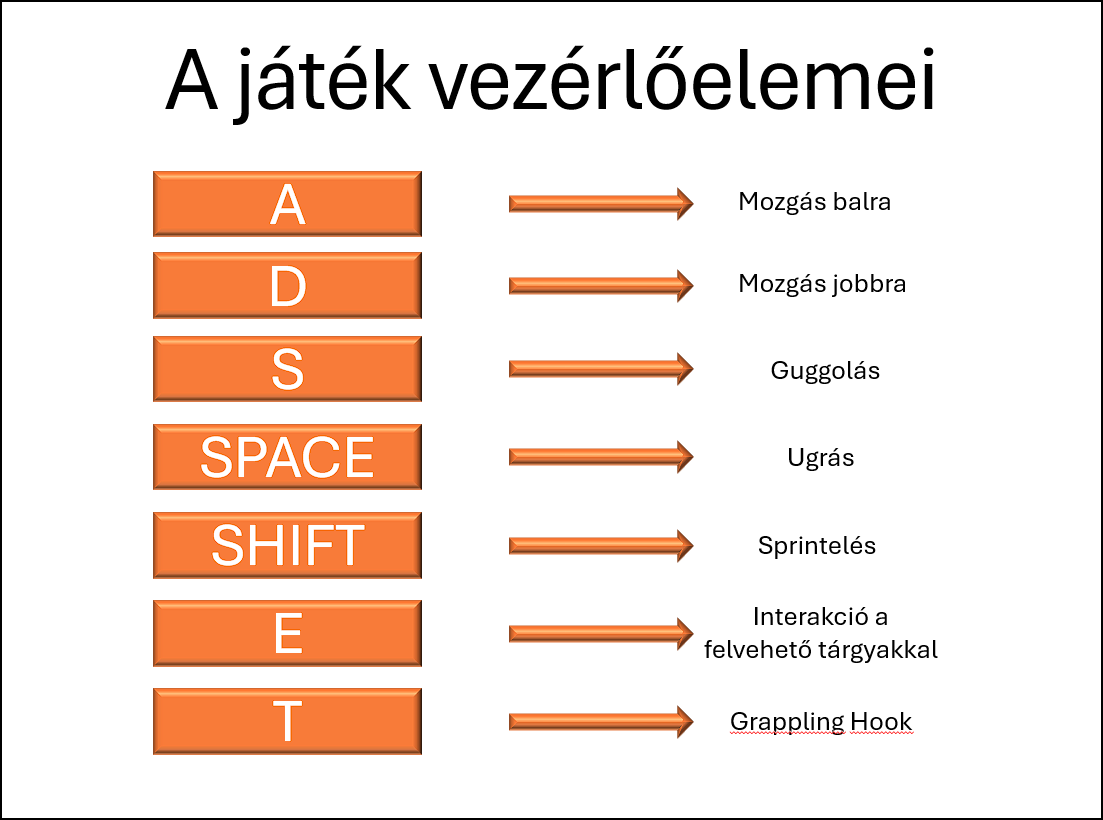
\includegraphics[scale = 0.3]{images/vezerloelemek.png}
\caption{A játék közben használt gombok és azok karakterakciói}
\label{fig:vezerloelemek}
\end{figure}

A játék több különböző szintből áll, amelyek mindegyike új kihívásokat és izgalmakat kínál a játékosoknak. A szintek száma és a szintek tervezése a játék fejlesztésének későbbi szakaszában lesz véglegesítve. A pályák kihívást jelentőek lesznek az akadályok elhelyezése révén. Ezek az akadályok különböző formákban és méretekben jelennek meg, és stratégiai gondolkodást igényelnek a játékosoktól a leküzdésükhöz. A játék egyik kiemelkedő funkciója a procedurális mapgenerálás, amely a főmenüben választható lesz. 

\Section{A Unity szerkesztője}

Amint megnyitjuk a Unity-t, a Unity Hub ablak fogad minket \cite{unityhub}. Itt tudunk projektet létrehozni, frissítéseket letölteni, valamint a Unity-t mint game engine-t jobban megismerni a Learn fül alatt. Miután létrehoztuk a projektünket, a Unity szerkesztője fogad majd minket, amelyet \aref{fig:unityszerkeszto}. ábrán láthatunk.

\begin{figure}[ht]
\centering
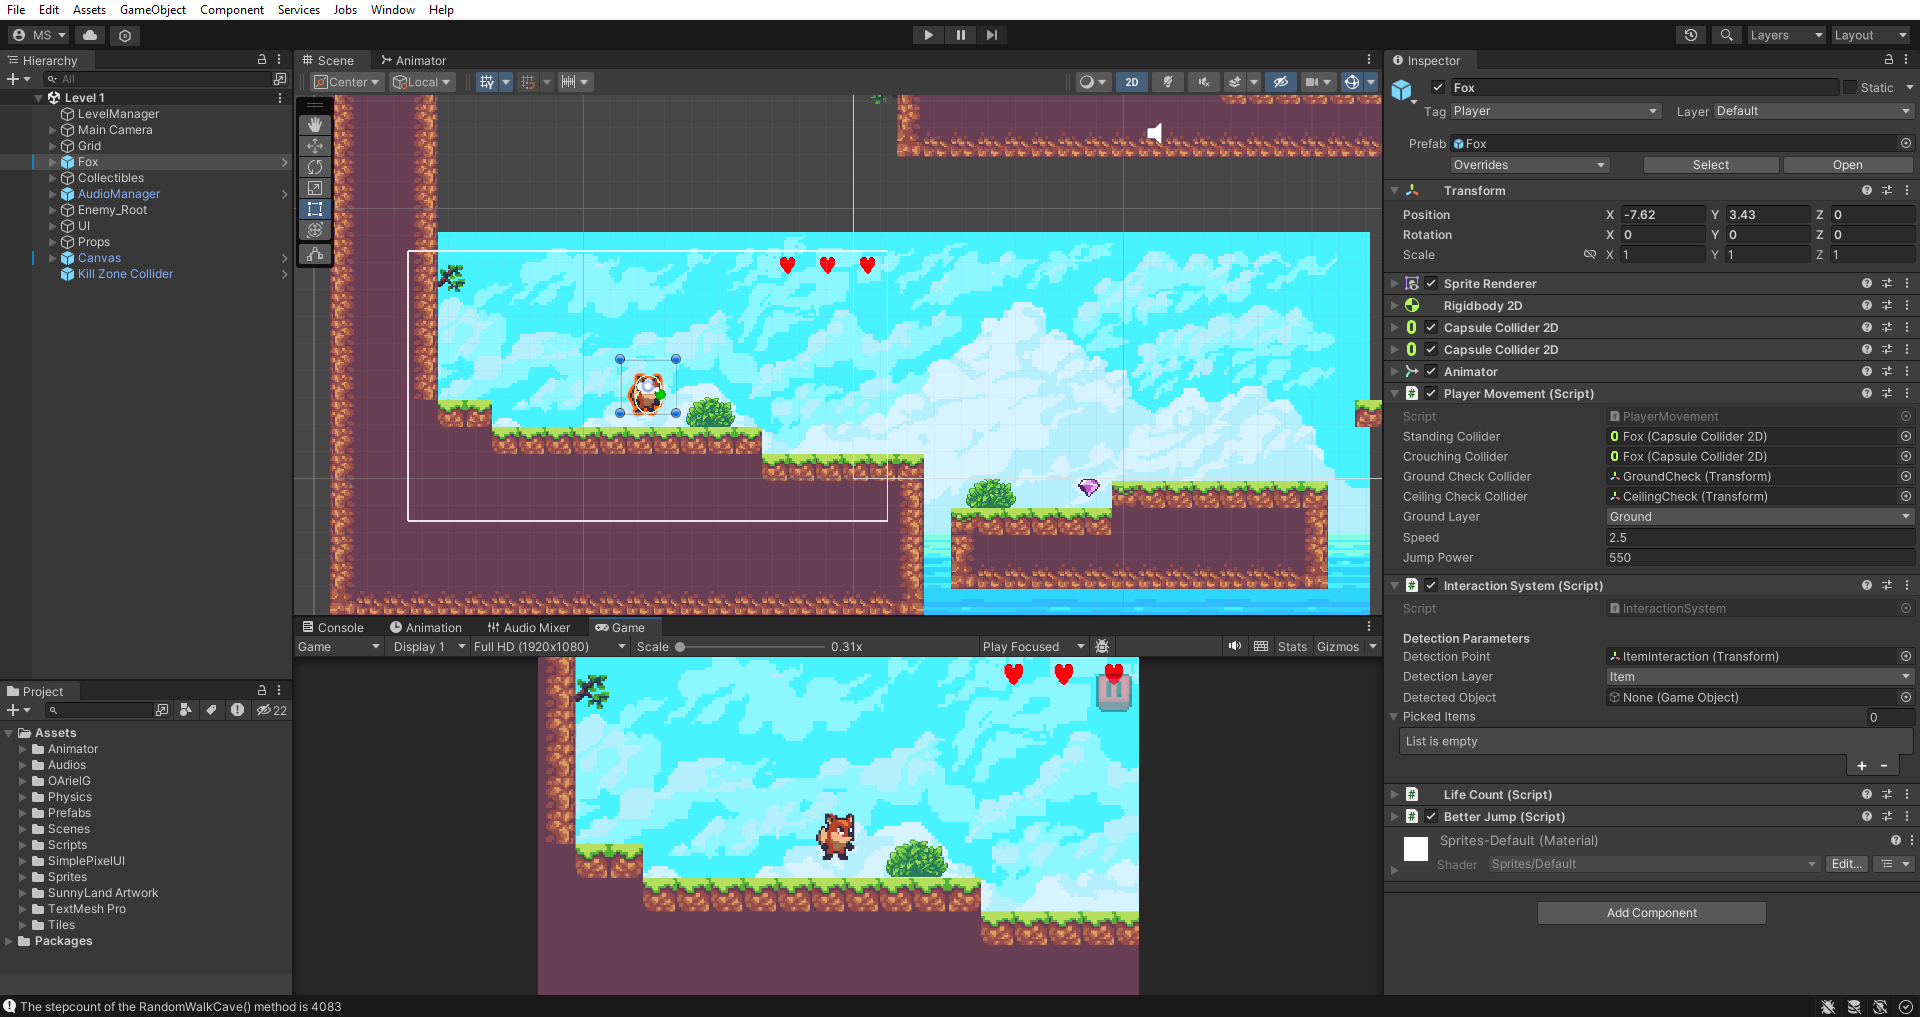
\includegraphics[width=\linewidth]{images/unityszerkeszto.png}
\caption{A Unity szerkesztője}
\label{fig:unityszerkeszto}
\end{figure}

A Hierarchy ablak azt a célt szolgálja, hogy felsorolja azokat a \texttt{GameObject}-eket, amelyek az aktuális Scene-en megtalálhatóak. A Project ablaknál találhatóak az Asset-ek, amelyeket az Asset Store-ból installálhatunk, valamint megtalálhatóak még az általunk kreált C\# szrkiptek, és a beimportált csomagok. Az Asset-ek a 2D-s vagy 3D-s modelleket, textúrákat, anyagjellemzőket tartalmazó fájlokat, háttereket, hangfájlokat jelentik, tulajdonképpen ezekből kreáljuk meg a játékunkat. A Console ablakon keresztül kommunikál a Unity a fejlesztővel, itt jelennek meg a \texttt{Debug.Log()} üzenetek, vagy a fordítási hibák. Az Animator és az Animation ablakok a \texttt{GameObject}-ek animálására szolgálnak. Megtalálható még az Inspector ablak, amely azt a célt szolgálja, hogy a kijelölt \texttt{GameObject}-hez kapcsolódó minden adat megtekinthető, változtatható legyen. Az ábrán látható még a Scene ablak, ahol a játékunk objektumait, hátterét és a pályát szerkeszthetjük. A Scene fül mellett található a Game ablak, ami kizárólag azt jeleníti meg, amelyet a Scene ablakban található kamera objektum lát.

\SubSection{4.2.1	A GameObject, valamint a szülő-gyerek kapcsolat}

A \texttt{GameObject} a Unity egyik legalapvetőbb objektuma. Képviselhet karaktereket, kellékeket, díszletet, kamerákat, útpontokat és még sok mást. Lényegében egy \texttt{GameObject} minden olyan objektum, amely elhelyezhető a \texttt{Scene} képernyőn. Fontos megjegyezni, hogy maga a \texttt{GameObject} nem sok mindent csinál; a hozzá csatolt komponensek adják meg a viselkedését, megjelenését és a célját. Például egy "Renderer" komponens hozzáadása láthatóvá teszi a \texttt{GameObject}-et, míg egy "Collider" komponens hozzáadása lehetővé teszi, hogy hasson rá a Unity fizikai motorja.\cite{unitygameobject}

A Unityben a \texttt{GameObject}-ek rendszerezése a scene-en belül hatékonyan egy szülő-gyermek hierarchián keresztül történik. Ez a hierarchikus, fára emlékeztető struktúra lehetővé teszi a \texttt{GameObject}-ek összekapcsolását. A szülő \texttt{GameObject} olyan tárolóként működik, amely hatással van a gyermekeire: a szülőre alkalmazott bármilyen transzformáció, például a mozgatás, forgatás vagy méretezés a gyermek \texttt{GameObject}-ekben is tükröződik. Minden gyermek \texttt{GameObject} a szülőjéhez kapcsolódik, és örökli annak transzformációs tulajdonságait. Ez azt jelenti, hogy ha a szülő mozog, a gyermek \texttt{GameObject} is mozogni fog, de megtartja azt a tulajdonságát, hogy függetlenül manipulálható. Például egy autó kerekei (gyermek \texttt{GameObject}-ek) önállóan is foroghatnak, miközben az autó (szülő \texttt{GameObject}) részei.\cite{unityhierarchy}

A hierarchikus rendszer különösen hasznos az összetett scene-ek kezelésében az összetartozó objektumok csoportosításában. Segít fenntartani a relatív pozíciókat egy objektum különböző összetevői között, amikor az egész objektum mozog. A hierarchia ráadásul különböző szinteken egymásba ágyazható, részletes és szervezett jelenetstruktúrát hozva létre.\cite{unityhierarchy} Például a \texttt{Collectibles} szülő \texttt{GameObject} és annak a \texttt{Diamond} gyermek \texttt{GameObject}-ei \aref{fig:hierarchydiamond}. ábrán látható.

\begin{figure}[ht]
\centering
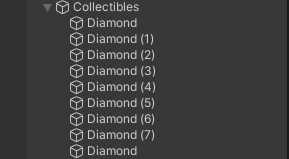
\includegraphics[scale = 1.0]{images/hierarchia.png}
\caption{A \texttt{Colletibles} objektum szülő-gyerek kapcsolatai}
\label{fig:hierarchydiamond}
\end{figure}

Ez a szülő-gyermek hierarchia a Unity tervezésének egyik alappillére, amely leegyszerűsíti a jelenetszervezést és biztosítja a kapcsolódó \texttt{GameObject}-ek közötti koordinált transzformációkat.

\Section{Az irányítható hős és a kamera}

Kezdetben be kell importálni az általunk kiválasztott assetet \cite{unityasset1} a Unity szerkesztőjébe, amelynek a neve SunnyLand. Ha ezt megtettük, akkor a \texttt{Project}fül alatt fogjuk látni a beimportált kellékeket, amelyekkel a játékunkat elkészítjük. A hierarchia ablaknál egyelőre csak a MainCamera \texttt{GameObject}-et látjuk, amely a nevéből is adódik, a fő kameránk. Ahhoz, hogy legyen egy irányítható karakterünk, előszőr a beimportált asset közül ki kell választani a karakterünk tétlen pozícióját reprezentáló Sprite-ot, majd egyszerűen a Scene ablakra kell húznunk, így létre is jön egy \texttt{GameObject}, amelynek tetszőleges nevet adhatunk. Az én esetemben a neve a Fox lett, mivel a karakterem egy róka.

Ha rámegyünk a Fox objektumra, akkor láthatjuk, hogy az első komponens az a \texttt{Transform} komponens. Ez minden egyes \texttt{GameObject}-hez automatikusan hozzá van rendelve, ez a Unity egyik legfontosabb komponense. Ezzel a komponenssel határozhatjuk meg az objektumunk helyzetét, forgását és a méretarányát. 
Az objektumunk helyzetét a „position” fülnél lévő X, Y és Z értékek változtatásával tudjuk megváltoztatni. A forgását a „rotation” fülnél levő szintén X, Y és Z értékek változtatásával tudjuk megváltoztatni. Végül, a „scale” opciónál lévő X, Y és Z értékek határozzák meg a \texttt{GameObject} méretét a jelenetben. 
Ezeket az értékeket szinte minden esetben manipulálják, változtatják és nem csak a Unity szerkesztőjében, hanem szkripteken keresztül is. \cite{transformcomponent}

A második komponens pedig a \texttt{Sprite Renderer} komponens, amely lényegében egy olyan eszköz a Unityben, amely a 2D-s képek megjelenítésére és kezelésére szolgál játék közben és nagyfokú ellenőrzést biztosít a képek megjelenítésének és interakciójának módjára. 

Ahhoz, hogy ezt a Fox objektumot fizikai alapú objektummá tegyük, hozzá kell adnunk a \texttt{Rigidbody2D} komponenst. A \texttt{Rigidbody2D} komponens a Unityben fizika alapú viselkedést ad a 2D-s sprite-okhoz. Amikor hozzáadjuk ezt a komponenst az objektumunkhoz, akkor a Unity ezt az objektumot a fizikai motorjának az irányítása alá vonja. Ez azt jelenti, hogy hatással lehetnek az objektumunkra különböző fizikai események, például a gravitáció. A \texttt{Rigidbody2D} átveszi az objektum mozgatásának irányítását a \texttt{Transform} komponenstől. Fontos, hogy a szkriptünkben a \texttt{Rigidbody2D}-t mozgassuk a \texttt{Transform} helyett a pontos fizikai szimulációk, valamint az ütközésérzékelés érdekében. Sok dolgot lehet változtatni a \texttt{Rigidbody2D} komponensen belül, mint például a test típusát, amelyet én dinamikusra állítottam annak érdekében, hogy ne lebegjen a levegőben a karakterem. \cite{unityrigidbody2d}

A másik dolog, amit át kellett állítanom az a „collision detection” érték, amelyet diszkrétről állítottam át folytonosra, hogy egyfolytában érzékelje az objektum, ha egy másik objektummal ütközik. A harmadik fontos dolog, hogy a korlátozások fül alatt lévő „Freeze Rotation Z” rublikát be kell pipálni, mert ha nem tesszük, akkor folyamatosan el fog dőlni a karakterünk.

 A következő komponens, amit hozzá kell adnunk az objektumunkhoz, az a \texttt{Capsule Collider2D}, amely egy kapszula alakú ütköztetőt biztosít, amely kölcsönhatásba lép a Unity 2D-s fizikai rendszeréve. Ha egy \texttt{Rigidbody2D} komponens is kapcsolódik ugyanahhoz a \texttt{GameObject}-hez, a \texttt{Capsule Collider 2D} lehetővé teszi, hogy az objektum fizikailag kölcsönhatásba lépjen a jelenet más objektumaival. Ez magában foglalja a gravitációra, erőkre és ütközésekre való reagálást. Ezt a komponenst kétszer kellett hozzáadnom az objektumhoz, mivel guggolásnál alacsonyabb méretű és  A talajhoz, amelyet kezdetben létrehoztam, ahhoz viszont a \texttt{Box Collider2D} komponenst kellett hozzáadnom.\cite{unityrigidbody2d} A Fox objektum komponensei \aref{fig:foxcomponents}. ábrán láthatóak.

\begin{figure}[ht]
\centering
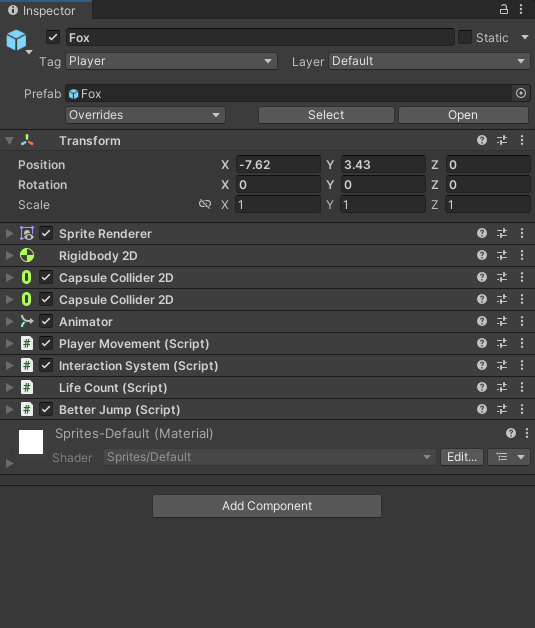
\includegraphics[scale = 0.7]{images/foxcomponents.png}
\caption{A Fox objektum komponensei}
\label{fig:foxcomponents}
\end{figure}

\newpage
\SubSection{A \texttt{PlayerMovement} osztály}

Ahhoz, hogy mozgásra bírjam a karakteremet, készítenem kell egy szkriptet. A \texttt{Project} ablakban létrehoztam egy „Scripts” nevű mappát, ahol létrehoztam egy C\# szkriptet \texttt{PlayerMovement} néven. Mielőtt bármit is programoznánk, először is a \texttt{PlayerMovement} szkriptet mint komponenst hozzá kell adnunk a Fox objektumunkhoz. A Unity automatikusan elkészíti nekünk a \texttt{PlayerMovement} osztályt, amely a \texttt{MonoBehaviour} osztályból örököl metódusokat. A \texttt{PlayerMovement} osztály osztálydiagramja \aref{fig:playermovementclass}. ábrán látható. 

\begin{figure}[ht]
\centering
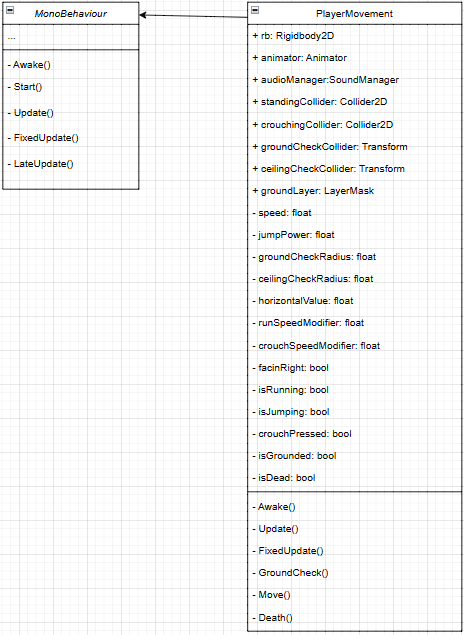
\includegraphics[scale = 0.8]{images/playerclass.png}
\caption{A \texttt{PlayerMovement} osztály osztálydiagramja}
\label{fig:playermovementclass}
\end{figure}

\newpage
Ilyen metódus például az \texttt{Awake()} metódus, amely akkor hívódik meg, amikor a jelenetünk betöltődik. Ez a metódus egyetlen egyszer fut le az élete során. A \texttt{Start()} metódus az \texttt{Awake()} metódushoz hasonlóan szintén egyszer fut le, azzal a különbséggel, hogy az \texttt{Awake()} hamarabb hívódik meg, ha mindkét metódus szerepel a programban. Ezeket csak olyan parancsokhoz érdemes használni, amelyeket csak egyszer szeretnénk lefuttatni. Például akkor, amikor referenciákat szeretnénk eltárolni komponens típusú változókban. A \texttt{Start()} metódus után következő \texttt{Update()} metódus is Unity által definiált, amely minden egyes képkockafrissítésnél hívódik meg. Ebből van több verzió, amelyek a \texttt{FixedUpdate()} és a \texttt{LateUpdate()}. A \texttt{FixedUpdate()} határozott időközönként kerül meghívásra, tehát független a képkockafrissítéstől. A \texttt{LateUpdate()} viszont képkockafrissítésenként hívódik meg, miután az \texttt{Update()} metódus már lefutott. 

Én az \texttt{Update()} és a \texttt{FixedUpdate()} függvényeket használtam. Az \texttt{Update()} függvény tartalmazza a \texttt{horizontalValue} inicializálását, a sebesség növelését amikor a karakter nem sétál hanem fut, valamint az ugrás és a guggolás parancsait is ebben a függvénybe helyeztem el. A karakterem „halotti állapotát” is az \texttt{Update()} függvényben kezelem le, ha az \texttt{isDead} változó értéke igaz, a metódus azonnal visszatér, kihagyva minden bemeneti feldolgozást. A \texttt{FixedUpdate()} függvényben hívom meg a \texttt{Move()} és a \texttt{GroundCheck()} metódusokat. Az alábbi metódus a \cite{youtubeplaylist} videósorozat alapján készült.

\begin{java}
 void Update()
 {
     if(isDead) return;

     //Values between -1 and 1 
     horizontalValue = Input.GetAxisRaw("Horizontal");

     //If leftshift is clicked, enable isRunning
     if(Input.GetKeyDown(KeyCode.LeftShift))
     {
         isRunning = true;
     }
     //if leftshift is released, disable isRunning
     if (Input.GetKeyUp(KeyCode.LeftShift))
     {
         isRunning = false;
     }
     if (Input.GetButtonDown("Jump"))
     {
         animator.SetBool("Jump", true);
         isJumping = true;
     }
     else if (Input.GetButtonUp("Jump"))
     {
         isJumping = false;
     }
     if (Input.GetButtonDown("Crouch"))
     {
         crouchPressed = true;
     }
     else if (Input.GetButtonUp("Crouch"))
     {
         crouchPressed = false;
     }

     //Set the y velocity in the animator
     animator.SetFloat("yVelocity", rb.velocity.y);

 }

 void FixedUpdate()
 {
     GroundCheck();
     Move(horizontalValue,isJumping,crouchPressed);
 }
\end{java}

A továbbiakban a \texttt{PlayerMovement} osztály metódusait fogom részletezni.

A \texttt{GroundCheck()} metódussal azt vizsgálom, hogy a Fox objektum egyik gyermek objektuma, a \texttt{GroundCheck}  objektum ütközik-e más, a „Ground” rétegben lévő 2DCollider-ekkel. A \texttt{wasGrounded} változó az \texttt{isGrounded} változó előző állapotát tárolja. Az \texttt{OverlapCircleAll()} metódus a Unity Physics2D-t használja annak ellenőrzésére, hogy a \texttt{groundCheckCollider} átfedésben van-e a \texttt{groundLayer} bármelyik ütközőjével. Ez az ellenőrzés a \texttt{groundCheckRadius} által meghatározott körön belül történik. Ezt a metódust egyenlővé tettem a \texttt{Colliders2D[]} típusú \texttt{colliders} nevezetű változóval, hiszen ha átfedés történik, akkor ez a metódus egy 0-nál nagyobb számmal tér vissza. Ha a \texttt{colliders} értéke nagyobb mint 0, akkor az \texttt{isGrounded} értékét igazra állítom, valamint, ha a levegőből érkezett a földre a karakterem, akkor egy landolási hangeffekt kerül lejátszásra. Ha a \texttt{colliders} értéke egyenlő a 0-val, akkor az \texttt{isGrounded} értéket hamisra állítom. A metódus végén a \texttt{Jump} animátor paramétert hamisra állítom, hogy az ugrás animáció leálljon. Az alábbi metódus a \cite{youtubeplaylist} videósorozat alapján készült.

\begin{java}
void GroundCheck()
{
    bool wasGrounded = isGrounded;

    //Checking if GroundCheckCollider collides
    //with other 2D Colliders that are in the "Ground" layer
    //If yes (isGrounded true) else (isGrounded false)
    Collider2D[] colliders = 
        Physics2D.OverlapCircleAll
        (groundCheckCollider.position, 
        groundCheckRadius,groundLayer);
    if (colliders.Length > 0)
    {
        isGrounded = true;
        if (!wasGrounded)
        {
            audioManager.PlaySFX(audioManager.landing);
        }

    }
    else
    {
        isGrounded = false;
    }    

    //As long as we're grounded
    //the jump bool in the animator is disabled.
    animator.SetBool("Jump", !isGrounded);
}
\end{java}

A \texttt{Move()} metódus tartalmazza a karakter X és Y tengelyen való mozgatását, hogyha a karakter földön van és megnyomjuk a SPACE billentyűt, akkor ugorjon, valamint azt is, hogyha a karakter megnyomjuk az S billentyűt, akkor guggoljon. Egy objektumot többféle módon mozgathatunk a programon belül. Egy objektum Transform komponensét elérhetjük a \texttt{gameObject.transform} osztályon keresztül, ezen belül több lehetőség is van, például a \texttt{position}-, a \texttt{localScale}-, a \texttt{velocity} tulajdonság vagy a \texttt{Translate()} metódus.

A \texttt{Jumping\&Crouching} részben először ellenőrzöm, hogy a \texttt{crouchFlag} értéke aktív-e. Ha nem aktív, akkor a \texttt{Physics2D.OverlapCircle} segítségével leellenőrzöm, hogy van-e olyan ütköző, amely átfedésben van a megadott pozícióba rajzolt körrel, amelynek a sugara a \texttt{ceilingCheckRadius} változó. Ha az ellenőrzés során bármilyen ütközőt találunk, vagyis valami közvetlenül a Fox objektum fölött van, akkor a \texttt{crouchFlag} igaz értéket kap. Ez gyakorlatilag guggoló helyzetben tartja a játékost, amíg egy olyan platform alatt van, amely ütközik a \texttt{CeilingCheck} objektummal. A következő fő blokk ellenőrzi, hogy a játékos földön van-e. Ha igen, akkor feldolgozza az ugrás és a guggolás mechanikáját.

 A guggolás mechanikája a következő: ha a \texttt{crouchFlag} igaz (mely értéket az S billentyű vagy a fentebb említett feltétel vált ki), akkor a \texttt{standingCollider.enabled} értéket hamisra állítom. A guggolás az \texttt{animator.SetBool(„Crouch”, crouchFlag)} segítségével kapcsolható ki és be. Ha a \texttt{crouchFlag} értéket igaz, akkor a guggolás animáció lejátszódik, ha hamis, akkor viszont nem. Az ugrás mechanizmusa a következő: még mindig az ellenőrzésen belül, hogy a játékos a földön tartózkodik-e, ha a \texttt{jumpFlag} értéke igaz (melyet jellemzően egy ugrás billentyű, esetemben a szóköz vált ki), több művelet is történik. Az egyik az, hogy az \texttt{isGrounded} értékét hamisra állítom, ezzel jelezve, hogy a játékos ugrást kezdeményezett, és már nem érintkezik a talajjal. Ezután az \texttt{audioManager.PlaySFX(audioManager.jumping)} metódus segítségével egy ugrás hanghatás kerül lejátszásra. A Rigidbody2D komponensre egy felfelé ható erő fog hatni a \texttt{rb.AddForce(new UnityEngine.Vector2(0f, jumpPower))} metódus által. A \texttt{Vector2} itt úgy van felépítve, hogy az x értékhez nincs erő rendelve, az y értékhez viszont a \texttt{jumpPower} értéket rendelem hozzá, ami függőlegesen fogja felfele tolni a Fox objektumot. Miután lekezeltem az ugrás és a guggolás feltételeit, ismét beállítom a \texttt{standingCollider} és a \texttt{crouchingCollider} aktív állapotait. A \texttt{standingCollider} le van tiltva, ha a \texttt{crouchFlag} értéke igaz, ellenkező esetben pedig engedélyezve van. A \texttt{crouchingCollider} engedélyezve van, ha a \texttt{crouchFlag} igaz, és le van tiltva, ha a \texttt{crouchFlag} hamis. Ez azért szükséges, mivel a Fox objektumon kettő darab CapsuleCollider2D található (\texttt{standingCollider} és a \texttt{crouchingCollider}), és ha a játékos ütközne egy ellenséggel, akkor kettő életerőt venne le a játékostól 1 helyett, mivel mindkét komponenssel ütközne az ellenfél. Az alábbi metódus a \cite{youtubeplaylist} videósorozat alapján készült.

\begin{java}
#region Jumping&Crouching
if (!crouchFlag)
{
    if (Physics2D.OverlapCircle
        (ceilingCheckCollider.position,
        ceilingCheckRadius,groundLayer))
    {
        crouchFlag = true;
    }
}

if (isGrounded)
{
    //If we press 'S' we disable the standing collider
    //and animate crouching
    //Reduce the speed by half
    //if released resume the original speed
    //enable the standing collider + disable crouch animation
    standingCollider.enabled = !crouchFlag;
    //If the player is grounded and pressed space -> Jump
    if (jumpFlag)
    {
        isGrounded = false;
        audioManager.PlaySFX(audioManager.jumping);
        //Add jump force
        rb.AddForce(new UnityEngine.Vector2(0f, jumpPower));
    }
    
}

animator.SetBool("Crouch", crouchFlag);
standingCollider.enabled = !crouchFlag;
crouchingCollider.enabled = crouchFlag;
#endregion
\end{java}

A \texttt{Move\&Run} részben a karakterem horizontális mozgását, valamint orientációját valósítottam meg. Kezdetben a vízszintes sebesség, melyet az \texttt{xVal} változó jelöl, úgy kerül kiszámításra, hogy a dir változót megszorozzuk a \texttt{speed} attribútummal, majd ezt tovább szorozzuk 100-zal, hogy a Unityben használható sebességskálára konvertáljuk, és a \texttt{Time.fixedDeltaTime} segítségével beállítjuk a képkockafrissítési függetlenségét. Ez a sebesség módosul annak alapján, hogy a játékos fut vagy guggol: megduplázódik, ha a játékos fut, amit az \texttt{isRunning} flag jelez, és megfeleződik, ha guggol, a \texttt{crouchFlag} alapján. A kiszámított sebességet ezután a Rigidbody2D-re alkalmazzuk, beállítva annak vízszintes komponensét a meglévő függőleges komponens megtartása mellett, ami lehetővé teszi a gravitációs hatások zavartalan érvényesülését. Ezután a játékos orientációját fogom kezelni a mozgási irány alapján. Ha a játékos irányt vált, a Fox objektumon lévő sprite megfordul, hogy a megfelelő irányba nézzen. Ez úgy történik, hogy a Transform komponens \texttt{localScale.x} tulajdonságát -1 vagy 1 értékre állítjuk, így a sprite az x tengelyen szükség szerint tükrözve lesz. Végül frissítem az \texttt{xVelocity} paramtért az Animator-ban, hogy tükrözze a Rigidbody aktuális x sebességének abszolút értékét. Ez az érték döntő fontosságú a séta- és futásanimációk vezérléséhez, hogy azok megfeleljenek a karakter tényleges mozgási sebességének. Az alábbi metódus a \cite{youtubeplaylist} videósorozat alapján készült.

\begin{java}
    #region Move & Run
    float xVal = dir * speed * 100 * Time.fixedDeltaTime;
    if(isRunning)
    {
        xVal *= runSpeedModifier;
    }
    if (crouchFlag)
    {
        xVal *= crouchSpeedModifier;
    }
    UnityEngine.Vector2 targetVelocity = 
        new UnityEngine.Vector2(xVal,rb.velocity.y);
    rb.velocity = targetVelocity;

    //IF looking right and clicked left ( flip to the left )
    if(facingRight && dir < 0)
    {
        transform.localScale = 
            new UnityEngine.Vector3(-1, 1, 1);
        facingRight = false;
    }
    // if looking left and clicked right ( flip to the right)
    else if (!facingRight && dir > 0) 
    {
        transform.localScale = 
            new UnityEngine.Vector3(1, 1, 1);
        facingRight = true;   
    }
    // set the float xVelocity according to the x value
    // of the Rigidbody2D velocity
    animator.SetFloat("xVelocity",Mathf.Abs(rb.velocity.x));
    #endregion
\end{java}

A \texttt{Death()} metódus a játékos halálát kezeli. Az \texttt{isDead} változó értékének az igazra állítása a játékost halottnak jelöli, hogy megakadályozzuk a további bemeneti feldolgozást. Ezután meghívok egy \texttt{Restart()} nevezetű metódust, amely a LevelManager osztályban található, hogy újraindítsam a pályát, ahol a játékos meghalt. Az alábbi metódus a \cite{youtubeplaylist} videósorozat alapján készült.

\begin{java}
public void Death()
{
    isDead = true;
    FindObjectOfType<LevelManager>().Restart();
}
\end{java}

\SubSection{A BetterJump osztály}

Ezt az osztályt azért hoztam létre, hogy javítsam az ugrás mechanikáját úgy, hogy a Rigidbody2D sebességét a játékos cselekvései és az ugrás állapota alapján sokkal élethűbbre állítom, mivel a karakterem ugrása kezdetben eléggé furcsának, természetellenesnek tűnt. Ez azért van egyébként, mivel más videójátékokban is a gyorsabb landolás a megszokott, és nem a „lebegős” ugrás. Az igazság az az, hogy a kezdetben implementált ugrás fizikailag helyes, hiszen azt az elképzelést követi, hogy bármennyi időbe telik is az, hogy az ugrásunk csúcsára érjünk, ugyan annyi időbe telik, amíg visszaérünk a földre. \cite{betterjump}

\begin{figure}[ht]
\centering
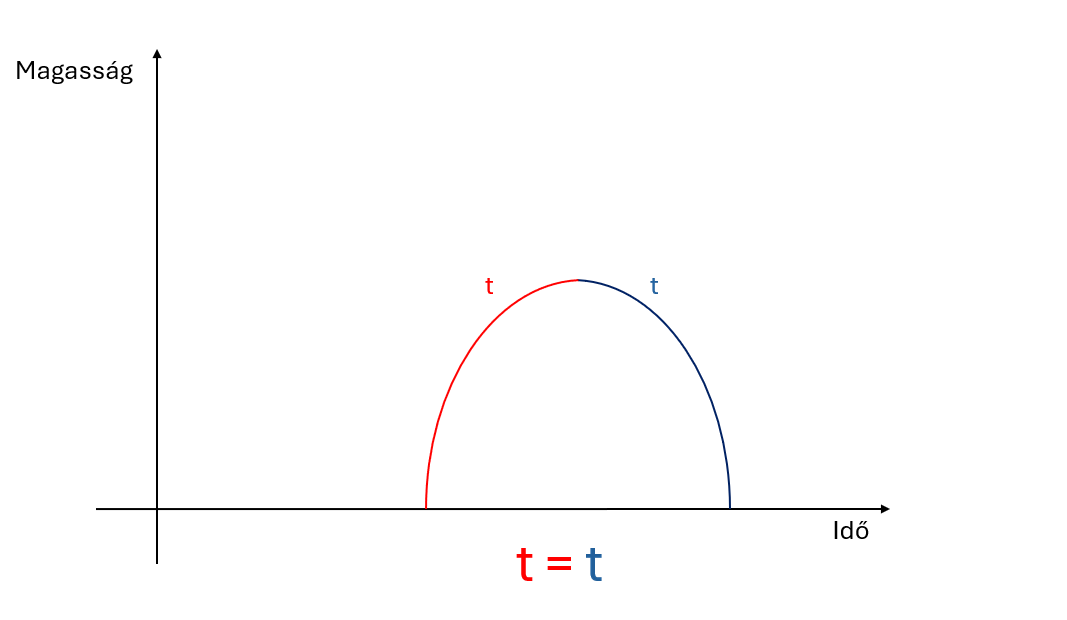
\includegraphics[width=\linewidth]{images/betterjumpgraph.png}
\caption{Az ugrás és a földet érés időtartama\cite{betterjump}}
\label{fig:betterjumpgraph}
\end{figure}

A videójátékokban ezt teljesen másképp kezelik. Az előbb leírt elmélet azt feltételezi, hogy ugyan annyi képkocka elérni a csúcsot, mint elérni a talajt. Azt kell tehát elérni, hogy több időt töltsön a levegőben a karakter amikor felfelé megy, mint amikor lefelé. Ezt a gravitáció manipulálásával lehet elérni.\cite{betterjump}

Először is létrehozok egy \texttt{Rigidbody2d} típusú \texttt{rb} nevű változót, amely a Rigidbody2D komponensre fog hivatkozni. Utána létrehozok két darab publikus \texttt{float} típusú változót, a \texttt{fallMultiplier}-t és a \texttt{lowJumpMultiplier}-t, amelyek segítségével be fogom tudni állítani a karakteremre ható gravitációs erőt eséskor és alacsony ugráskor (olyan ugrás, amikor az ugrás gombot gyorsan elengedjük), így az ugrás vagy erőteljesebb vagy kevésbé erőteljes lesz. Az \texttt{Awake()} metódusban a szkript megkapja a Rigidbody2D komponenst a \texttt{GameObject}-ből, amelyhez a szkript csatlakozik, és az \texttt{rb} változóban tárolja.

Az \texttt{Update()} metódus aktívan figyeli a játékos ugrási feltételeit, hogy módosításokat alkalmazzon az ugrás fizikájában. Ha a karakter zuhan –- amit a játékos sebességében lévő y-komponens jelez --, a szkript növeli a gravitációs erő vonzását. Ez úgy történik, hogy a Rigidbody sebességét a \texttt{Vector2.up} és a \texttt{Physics2D.gravity.y}, valamint a beállított \texttt{fallMultiplier} szorzataként kiszámított és a \texttt{Time.deltaTime} értékkel skálázott hozzáadott erővel módosítja. Ez a képlet jelentősen felgyorsítja a játékos esését az ugrás csúcspontjának elérése után, így valósághűbb és kielégítőbb esést lehet biztosítani.

Ezzel szemben, ha a játékos ugrik, és gyorsan elengedi az ugrás gombot (ezek a pozitív y-sebességgel és az „ugrás” gomb megnyomásának hiányával észlelhető), alacsony ugrást fog eredményezni. Ezt úgy lehet elérni, hogy a \texttt{lowJumpMultiplier} segítségével kissé növeljük a gravitációt, ami csökkenti az emelkedés meredekségét és gyorsítja az ereszkedést. Ez a feltétel lehetővé teszi, hogy gyors, kevésbé erőteljes ugrásokat hajtsanak végre a játékosok. Az alábbi osztály a \cite{betterjump} videó alapján készült.

\begin{java}
public class BetterJump : MonoBehaviour
{
    public float fallMultiplier = 2.5f;
    public float lowJumpMultiplier = 2f;

    Rigidbody2D rb;

    private void Awake()
    {
        rb = GetComponent<Rigidbody2D>();
    }

    private void Update()
    {
        if(rb.velocity.y < 0) 
        {
            rb.velocity += 
                Vector2.up * Physics2D.gravity.y * 
                (fallMultiplier - 1) * Time.deltaTime;
        }
        else if(rb.velocity.y > 0 && !Input.GetButton("Jump"))
        {
            rb.velocity += 
                Vector2.up * Physics2D.gravity.y * 
                (lowJumpMultiplier - 1) * Time.deltaTime;
        }
        
    }
}
\end{java}

\SubSection{A Grappling Hook mechanizmus}

A grappling hook mechanizmus a videójátékokban általában egy kötél, amelyre egy csáklya vagy valamilyen karommal rendelkező eszköz van ráerősítve, majd ezt a játékokban kilövik vagy eldobják, amely megakad a célpontban, és odahúzza a játékost az célponthoz, vagy a célpontot húzza oda a játékoshoz. A játékomban a játékost húzza majd oda a célponthoz, azaz egy falhoz, mivel csak a tile-okhoz tudja majd magát odahúzni a játékosom. Ezt a mechanizmust azért építettem bele a játékba, hogy a procedurálisan generált pályát a játékosom végig tudja vinni.

Ahhoz, hogy létre tudjam hozni ezt a játékmechanikát, a Fox objektumomhoz hozzá kellet csatolnom egy úgynevezett \texttt{Distance Joint 2D} komponenst, valamint létre kellett hoznom egy üres \texttt{GameObject}-et, amelynek a \texttt{Rope} nevet adtam. Ehhez a \texttt{Rope} objektumhoz hozzá kellett adnom a \texttt{Line Renderer} komponenst, hogy vizuálisan is látni lehessen a kötelet, amelyet majd a Fox objektum pozíciójából a T betű lenyomására kilő a játékos. Ahhoz, hogy a játékos oda tudja magát húzni a megcélzott falhoz, vagy platformhoz, egy szkriptet kellett írjak.

Ennek a szkriptnek a neve Grappling Hook. Ez a szkript a Fox \texttt{GameObject}-hez van csatolva, mivel innen fogja kilőni a játékos a kötelet.

\textbf{Inicializáció:}
\begin{itemize}
\item \texttt{LineRenderer line}: A 2D térben pontok közötti vonalakat rajzoló vizuális komponens. Itt a grappling hook kötelének renderelésére használom.
\item \texttt{DistanceJoint2D joint}: Fizikai komponens, amely két pontot meghatározott távolságra tart egymástól. Ebben az esetben biztosítja, hogy a játékos és a grappling hook horgonya meghatározott távolságot tartson.
\item \texttt{Vector3 targetPos}: A grappling hook célpozícióját tárolja, ahová az egérkurzor mutat, amikor a játékos aktiválja a horgot.
\item \texttt{RaycastHit2D hit}: Tárolja az információt arról, hogy a raycast mit talál el, ami annak meghatározására szolgál, hogy a grappling hook tud-e valamire rögzülni.
\item \texttt{LayerMask layerMask}: Megszűri, hogy a raycast milyen objektumokat találhat el, javítva ezzel a teljesítményt és biztosítva, hogy a grappling hook csak olyan objektumokkal lépjen kölcsönhatásba, amelyekkel kell.
\item \texttt{public float distance}: Azt határozza meg, hogy a grappling hook milyen messzire érjen el
\item \texttt{public float step}: Azt határozza meg, hogy a grappling hook milyen gyorsan húzódjon vissza.
\end{itemize}

A \texttt{Start()} metódussal inicializálom a \texttt{DistanceJoin2D}-t, majd ezután letiltom a \texttt{LineRenderer} komponenst, mivel a grappling hook kezdetben nem aktív. Az \texttt{Update()} metódus folyamatosan ellenőrzi, hogy a grappling hook aktív-e, és a távolság alapján beállítja a hosszát vagy leállítja, frissíti a kötél vizuális megjelenítését, hogy kövesse a játékost, valamintf igyel a játékos bemenetére a kapaszkodási művelet elindításához és leállításához.

A \texttt{StartGrappling()} metódus átalakítja az egér pozícióját világkoordinátákká, és ellenőrzi, hogy van-e érvényes célpont a grappling hook rögzítéséhez egy raycast segítségével. Ha érvényes célpontot talál, létrehoz egy új \texttt{GameObject}-et, amely a grappling hook horgonypontjaként szolgál, és hozzácsatolja a \texttt{DistanceJoint2D}-t. Ennek az objektumnak a létrehozásához azért volt szükség, mivel a \texttt{DistanceJoint2D} csak olyan objektumhoz tud hozzácsatlakozni, amely rendelkezik \texttt{Rigidbody2D} komponennsel. A platformok viszont nem rendelkeznek \texttt{Rigidbody} komponenssel. Ezután beállítja a vizuális vonalat a játékostól a célpontig. Az alábbi metódus a \cite{grapplinghook1} és a \cite{grapplinghook2} videók alapján készült.

\begin{java}
void StartGrappling()
{
    targetPos = 
        Camera.main.
        ScreenToWorldPoint(Input.mousePosition);
    targetPos.z = 0;
    hit = 
        Physics2D.Raycast(
            transform.position, 
            targetPos - transform.position, 
            distance, layerMask);

    if (hit.collider != null)
    {
        if (hit.collider.gameObject.
            GetComponent<TilemapCollider2D>() != null || 
            hit.collider.gameObject.
            GetComponent<Rigidbody2D>() != null)
        {
            GameObject anchor = 
                new GameObject("GrappleAnchor");
            anchor.transform.position = hit.point;
            Rigidbody2D anchorRb = 
                anchor.AddComponent<Rigidbody2D>();
            anchorRb.bodyType = 
                RigidbodyType2D.Static;

            joint.enabled = true;
            joint.connectedBody = anchorRb;
            joint.connectedAnchor = Vector2.zero;
            joint.distance = 
                Vector2.Distance(transform.position, 
                hit.point);
            line.enabled = true;
            line.SetPosition(0, transform.position);
            line.SetPosition(1, hit.point);
        }
    }
}
\end{java}

\SubSection{A MainCamera objektum és a hozzá tartozó szkript}

A \texttt{MainCamera} objektum az egyik legfontosabb eleme bármelyik projektnek, hiszen a játékos ezen keresztül látja a játékvilágot. A főkamera a játékos szemeként működik a játékkörnyezetben, és megjeleníti a képernyőn megjelenő dolgokat. Minden, ami a kamera látóterében van, az az, amit a játékos láthat a játékban. A Unity kamerái perspektivikus vagy ortografikus vetítést használhatnak. A perspektivikus vetítés az emberi szem látásmódját utánozza, a távolabbi elemek kisebbnek tűnnek, míg a közelebbi objektumok nagyobbnak. Az ortografikus vetítés az objektumokat a kamerától való távolságuktól függetlenül azonos méretben jeleníti meg, ami a 2D-s játékokban nagyon gyakori. Perspektivikus kamerák esetében a látómező (Field of View) határozza meg a megfigyelhető világnak a kiterjedését. A kamerák szkriptek segítségével konfigurálhatók és manipulálhatók, annak érdekében, hogy például kövessék a játékost, filmszerű effekteket hozzanak létre vagy reagáljanak a játék eseményeire, növelve a játék interaktivitását és dinamikáját. A Unity lehetővé teszi több kamera használatát a játékjelenet különböző részeinek egyidejű rendereléséhez. Például az egyik kamera beállítható a játékmenethez, míg egy másik megjelenítheti a felhasználói felületet vagy a speciális effekteket. A Unity ezeket a nézeteket egymásra rétegezi, és így hozza létre a végső képet, amelyet a játékos lát. Az Audio Listener komponens jellemzően a \texttt{MainCamera} objektumhoz kapcsolódik, és a jelenetben elhelyezett hangforrásokkal együtt működik.\cite{cameracomponent} A \texttt{MainCamera} objektum, valamint a hozzácsatolt komponensek \aref{fig:maincamera}. ábrán látható.

\begin{figure}[ht]
\centering
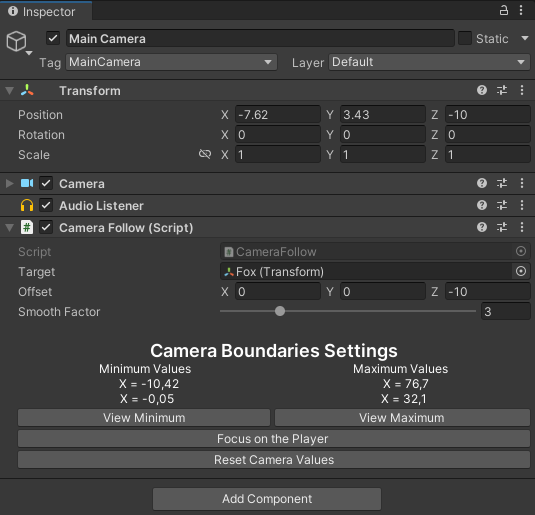
\includegraphics[scale = 0.6]{images/maincameracomponents.png}
\caption{A \texttt{MainCamera} objektum és komponensei}
\label{fig:maincamera}
\end{figure}

Ha a hierarchiában ráhúzzuk a kamerát a karakter objektumra, így létrehozva a szülő gyerek kapcsolatot, a kamera követni fogja a játékost. Ekkor a kamera transform értékeit átírva megadhatjuk, hogy mennyire legyen eltolva és elforgatva a karakterhez képest. Kezdésnek ez is elég jó eredményt ad, de amikor már komplexebb mozgásokat szeretnénk megadni a kamerának, programot kell rá írni.

Ezért létrehoztam egy CameraFollow szkriptet, ami a játék kamerájának a mozgásáért, valamint a határainak a beállításáért felel. Létrehoztam egy \texttt{public Transform} típusú, \texttt{target} nevű változót, amely referenciát fog tárolni a Fox objektumról. A \texttt{Vector3 offset} vektor a célpont és a kamera közötti eltolás annak érdekében, hogy a kamera ne legyen közvetlenül a célpont tetején. A \texttt{float smoothFactor} változó a kamera mozgásának az egyenletességét határozza meg. A \texttt{Vector3 minValues} és a \texttt{Vector3 maxValues} vektorok a kamera pozíciójának a minimális és maximális értékeit határozza meg, a kamera mozgását egy adott területre korlátozva. 

Az alább látható a \texttt{Follow()} metódus, aminek a  célja, hogy zökkenőmentesen kövessen egy célpontot meghatározott határokon belül. A módszer azzal kezdődik, hogy a target aktuális pozíciója alapján meghatározza, hogy a kamerát ideális esetben hová kellene pozícionálni. Hozzáad egy előre meghatározott \texttt{offset}-et a célpont pozíciójához, ami lehetővé teszi, hogy a kamera a célponttól állandó távolságot tartson, ahelyett, hogy közvetlenül a célponton ülne. Ez az eltolás különösen hasznos annak biztosításához, hogy a kamera jó rálátást biztosítson az eseményekre, a karaktert a képen tartva, miközben elegendő részt mutat a környezetből. 

A target pozíciójának kiszámítása után a módszer úgy korlátozza ezt a pozíciót, hogy a megadott minimális (\texttt{minValues}) és maximális (\texttt{maxValues}) határértékeken belül maradjon. Ez a \texttt{Mathf.Clamp} segítségével történik, amely a célpozíciót az egyes tengelyekre (\texttt{x, y, z}) vonatkozó \texttt{minValues} és \texttt{maxValues} által meghatározott tartományra korlátozza. Ez a rögzítés biztosítja, hogy a kamera ne mozduljon ki a játékvilág tervezett területéről, például ne mozogjon a szint szélein túl, vagy olyan területekre, ahol nem történik játék.

A kamera végső pozícióját a \texttt{Vector3.Lerp} függvény segítségével számítjuk ki. Ez a függvény lineárisan interpolál a kamera aktuális pozíciója (\texttt{transform.position}) és a korlátozott célpozíció (\texttt{boundPos}) között egy simítási tényező (\texttt{smoothFactor}) alapján. Az interpoláció a \texttt{Time.fixedDeltaTime} értékkel szorzódik meg, hogy a mozgás sima és egyenletes legyen a különböző képkocka sebességek között. Az alábbi metódus a \cite{youtubeplaylist} videósorozat alapján készült.

\begin{java}
void Follow()
{
    //Define minimum x,y,z values and maximum x,y,z values

    Vector3 targetPosition = target.position + offset;
    // Verify if the target position is out or not
    //Limit it to the min and max values
    Vector3 boundPos = new Vector3(
        Mathf.Clamp
        (targetPosition.x, minValues.x, maxValues.x),
        Mathf.Clamp
        (targetPosition.y,minValues.y,maxValues.y),
        Mathf.Clamp
        (targetPosition.z,minValues.z,maxValues.z));

    Vector3 smoothPosition = 
        Vector3.Lerp
        (transform.position, boundPos, 
        smoothFactor * Time.fixedDeltaTime);
    transform.position = smoothPosition;
}
\end{java}

Miután elkészítettem a \texttt{Follow()} metódust, és beállítottam az első pályán a kamera határait, rájöttem, hogy eléggé időigényes, ezért elkezdtem keresgélni, hogy hogyan is lehetne egyszerűbben, és gyorsabban beállítani ezeket a határokat, mivel nem csak ez lesz az egyetlen szint a játékomban. A legjobbnak tűnő megoldás egy grafikus felhasználói felület elkészítése, amely az Inspector menüben, a CameraFollow szkriptnél jelenik meg. Az általam létrehozott GUI \aref{fig:gui}. ábrán tekinthető meg.

\begin{figure}[ht]
\centering
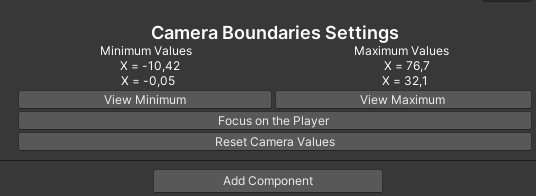
\includegraphics[scale = 0.9]{images/gui.png}
\caption{A \texttt{MainCamera} objektum általam létrehozott GUI része}
\label{fig:gui}
\end{figure}

\newpage
Ezt úgy készítettem el, hogy egy feltételes fordítási blokkban hoztam létre az egyéni szerkesztőfunkciókat. A \texttt{[CustomEditor(typeof(CameraFollow))]} sorral megadtam az alatta implementált osztálynak, hogy melyik futási idejű típusnak lesz a szerkesztője. Ez az osztály a \texttt{CameraFollowEditor}, amelynek a szülője nem a \texttt{MonoBehaviour}, hanem az \texttt{Editor} osztály. Ahhoz, hogy létrehozzak egy egyéni inspector-t, felül kell írjam az \texttt{OnInspectorGUI()} metódust, amelyet az \texttt{Editor} osztályból örököl az általam kreált \texttt{CameraFollowEditor} osztály.

A Unity \texttt{DrawDefaultInspector()} metódusát használtam annak a biztosítására, hogy a CameraFollow szkript minden nyílvános mezője látható és módosítható legyen. Ahhoz, hogy felhasználóbarát, és könnyed legyen a határok beállítása, különböző GUI-stílusokat és elrendezési elemeket használtam. Specifikus stílusokat határoztam meg, mind például a \texttt{defaultStyle}, amely az általános szöveg stílusáért felelős, valamint a \texttt{titleStyle}, ami pedig a szakaszcímekért felelős, így a felület sokkal áttekinthetőbbé és látványosabbá vált. Ezeket a stílusokat különböző interaktív GUI-elemekre, köztük címkékre és gombokra alkalmaztam, amelyek végig vezetnek a kamera konfigurációs folyamatán.

Ezek az interaktív elemek különösen hasznosak, hiszen a „View Minimum” és a „View Maximum” gombok lehetővé teszik, hogy az előre meghatározott határokhoz mozogjon a kamera, lehetővé téve a menetközbeni beállításokat és vizuális ellenőrzéseket. A további funkciók közé tartozik még a „Focus On The Player” gomb, amivel azonnal a játékosra írányíthatjuk a kamerát, valamint a „Reset Camera Values” gomb, amely a CameraFollow osztály \texttt{ResetValues()} metódusát hívja meg, amellyel töröl minden beállítást, és lehetővé teszi a határértékek beállításának az újrakezdését. Az alábbi kódrészlet a \cite{youtubeplaylist} videósorozat alapján készült.

\begin{java}
if (script.setupComplete) 
{
    GUILayout.BeginHorizontal();
    GUILayout.Label("Minimum Values",
        defaultStyle);
    GUILayout.Label("Maximum Values",
        defaultStyle);
    GUILayout.EndHorizontal();

    GUILayout.BeginHorizontal();
    GUILayout.Label($"X = {script.minValues.x}", 
        defaultStyle);
    GUILayout.Label($"X = {script.maxValues.x}", 
        defaultStyle);
    GUILayout.EndHorizontal();

    GUILayout.BeginHorizontal();
    GUILayout.Label($"X = {script.minValues.y}", 
        defaultStyle);
    GUILayout.Label($"X = {script.maxValues.y}", 
        defaultStyle);
    GUILayout.EndHorizontal();

    GUILayout.BeginHorizontal();
    if(GUILayout.Button("View Minimum"))
    {
        //Snap the cameraview to the min values.
        Camera.main.transform.position = script.minValues;
    }
    if(GUILayout.Button("View Maximum"))
    {
        //Snap the cameraview to the max values.
        Camera.main.transform.position = script.minValues;
    }
    GUILayout.EndHorizontal();

    if (GUILayout.Button("Focus on the Player"))
    {
        Vector3 targetPos = script.target.position;
        targetPos.z = script.minValues.z;
        Camera.main.transform.position = targetPos;
    }

    if (GUILayout.Button("Reset Camera Values"))
    {
        //Reset the setupcomplete bool
        //Reset the min max vec3 values
        script.ResetValues();
    }
\end{java}

Ezek az opciók azután jelennek meg, miután a grafikus felhasználói felület végigvitte a felhasználót egy struktúrált beállítási folyamaton. A beállítási folyamatnak három állapota van: a Step1, a Step2 és a None. Ha a kamerahatárértékek beállítása még nincs inicializálva (\texttt{if(script.state == CameraFollow.SetupState.None)}), akkor a szkript megjeleníti a „Start setting the camera values” gombot. Erre a gombra kattintva a beállítás állapot a „Step1” lesz, és elindul a határértékek beállításának a folyamata.

Az 1. lépést követően a szerkesztő felhasználói felületén utasítások jelennek meg, amelyek a kamera minimális határainak a konfigurálásának a lépései lesznek:
\begin{enumerate}
\item A „Select your Main Camera” felszólít minket, hogy a MainCamera legyen az aktív objektum a szerkesztőben
\item "Move it to the bottom left bound limit of your level" arra utasít, hogy manuálisan állítsuk be a kamera pozícióját a játékterület bal alsó sarkába, ahol a kamera határa kezdődik.
\item Kattintsunk a „Set min values” gombra. Erre a gombra kattintva rögzíti a főkamera aktuális pozícióját, és beállítja azt a minimális határértéknek.
\end{enumerate}
A kamerabeállítás lépései \aref{fig:camerasteps}. ábrán láthatóak.

\begin{figure}[ht]
\centering
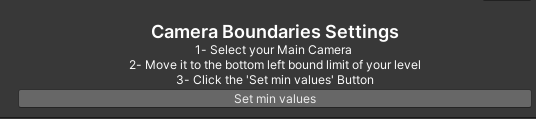
\includegraphics[scale = 0.9]{images/camerasteps.png}
\caption{A kamera minimumértékének beállítási lépései}
\label{fig:camerasteps}
\end{figure}

A minimális értékek beállítása után az állapot a második fázisba lép. Ez szinte ugyan az, mint az első fázis, annyi különbséggel, hogy maximális értékeket állítunk be. Ha beállítottuk a maximális értékeket, akkor a beállítás állapota visszatér a „None” állapotba, és a \texttt{script.setupComplete} igazra állítódik, jelezve, hogy a kamera határainak a beállítása befejeződött. A határértékek beállításáért felelős kódrészlet az alább megtekinthető. Az alábbi kódrészlet a \cite{youtubeplaylist} videósorozat alapján készült.

\begin{java}
if (script.state == CameraFollow.SetupState.None)
{
    if (GUILayout.Button("Start setting the camera values"))
    {
        //Changes the state to step1
        script.state = CameraFollow.SetupState.Step1;
    }
}
//Step 1: Set up the bottom left boundary (min values)
else if (script.state == CameraFollow.SetupState.Step1)
{
    //Instruction on what to do
    GUILayout.Label($"1- Select your Main Camera",
        defaultStyle);
    GUILayout.Label($"2- Move it to the bottom " +
        $"left bound limit of your level", defaultStyle);
    GUILayout.Label($"3- Click the 'Set min values' Button", 
        defaultStyle);

    //Button to set the min values
    if(GUILayout.Button("Set min values"))
    {
        //Set the min values of the cameralimit
        script.minValues = Camera.main.transform.position;
        //Change to step2
        script.state = CameraFollow.SetupState.Step2;
    }
}
//Step 2: Set up the top right boundary (max values)
else if (script.state == CameraFollow.SetupState.Step2)
{
    //Instruction on what to do
    GUILayout.Label($"1- Select your Main Camera", 
        defaultStyle);
    GUILayout.Label($"2- Move it to the top " +
        $"right bound limit of your level", defaultStyle);
    GUILayout.Label($"3- Click the 'Set max values' Button", 
        defaultStyle);

    //Button to set the min values
    if (GUILayout.Button("Set max values"))
    {
        //Set the min values of the cameralimit
        script.maxValues = Camera.main.transform.position;
        //Change to None
        script.state = CameraFollow.SetupState.None;
        //Last thing is to enable the setupComplete value
        script.setupComplete = true;
    }
}
\end{java}

\Section{Az irányítható karakter animálása}

Anélkül, hogy programot írnánk, a Unity képes animálás segítségével mozgatni objektumokat. Erre jó példa a játékomban például az ugrás, futás, landolás, guggolás, az ellenségek és az érmék animációi. Ezeket az animator controller valósítja meg, melyre gondolhatunk úgy, mint egy állapotgépre\cite{animatorcomponent}. Vannak állapotok, melyek egy-egy animációt reprezentálnak és vannak állapotátmenetek, melyek a végpontjaikban található animációkat felhasználva váltanak az egyik animációról a másikra. Ez a váltás történhet automatikusan, vagy paraméterek, küszöbértékek megadásával is.

Az \texttt{animator controller}-t tartalmazó objektum példányosítása után a kontroller a belépési állapottól egészen a kilépési állapotig fut az átmenetek mentén. Az állapotátmenetekkel megadhatjuk, hogy mely állapotokból mely állapotokba lehetséges a váltás. Egyik állapotból egy másik állapotba az átmenet (beállítástól függően) történhet automatikusan (például, ha az állapothoz tartozó animáció véget ért, mehetünk a másik állapotba), vagy paraméterek megadásával, melyeket programon belül állíthatunk be. Mindig csak egy állapot vagy egy átmenet lehet aktív a \texttt{controller}-ben. A Fox objektum \texttt{animator controller}-e \aref{fig:animatorcontroller}. ábrán megtekinthető.

\begin{figure}[ht]
\centering
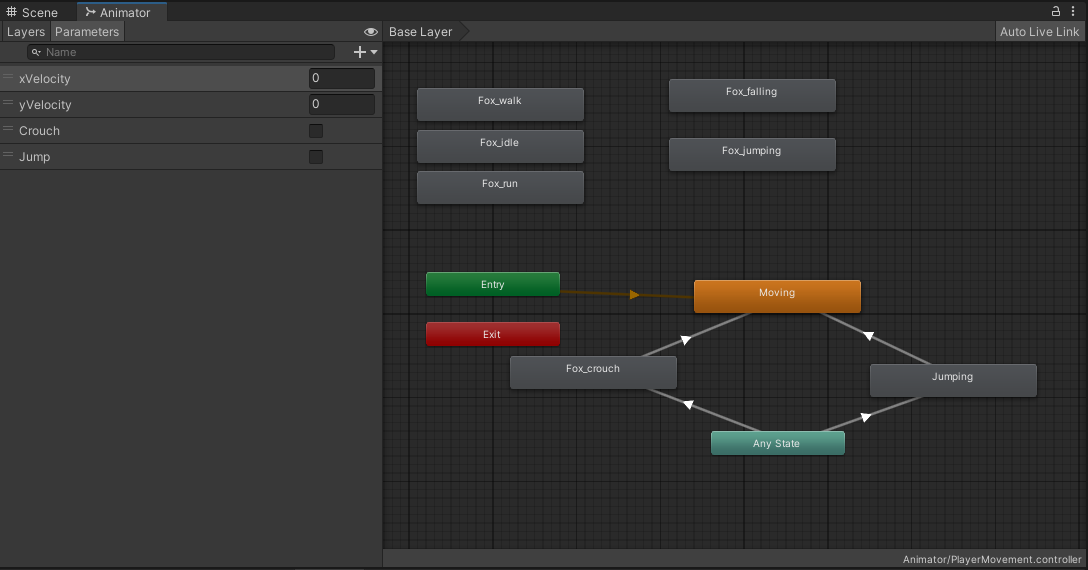
\includegraphics[scale = 0.5]{images/animatorcontroller.png}
\caption{A Fox GameObject animator controller-e}
\label{fig:animatorcontroller}
\end{figure}

Az \texttt{Entry} állapot a belépési pontot, az \texttt{Exit} állapot pedig a kilépési pontot jelenti. A \texttt{Moving} állapot pedig az alap állapot, amely egy \texttt{Blend Tree} melyben szerepelnek a fent lévő \texttt{Fox\_walk}, \texttt{Fox\_idle} és \texttt{Fox\_run} állapotok, amelyeket az Animation fül alatt lehet létrehozni Sprite-ok segítségével. Az \texttt{Any State} állapothoz tartozó animációk bármelyik állapot után aktiválódhatnak, ezért is kapcsolódik hozzá a \texttt{Fox\_crouch} és a \texttt{Jumping} állapot. A \texttt{Jumping} szintén egy \texttt{Blend Tree}, amelyben a \texttt{Fox\_falling} és a \texttt{Fox\_jumping} állapotok szerepelnek. Az Animator ablakon belül a Parameters fülnél lehet változókat definiálni, a Layers fül alatt pedig rétegeket létrehozni.

\newpage
A \texttt{Blend Tree}-t állapotgép helyett használtam annak érdekében, hogy különböző küszöbértékek megadásával váltakozzanak az \texttt{Fox\_idle}, a \texttt{Fox\_walk} és a \texttt{Fox\_run} animációk (ezek a \texttt{Moving Blend Tree}-ben láthatók), valamint az ugrásnál is ugyan ezt a szisztémát követtem. A \texttt{Moving} nevű \texttt{Blend Tree} \aref{fig:blendtree}. ábrán megtekinthető.

\begin{figure}[ht]
\centering
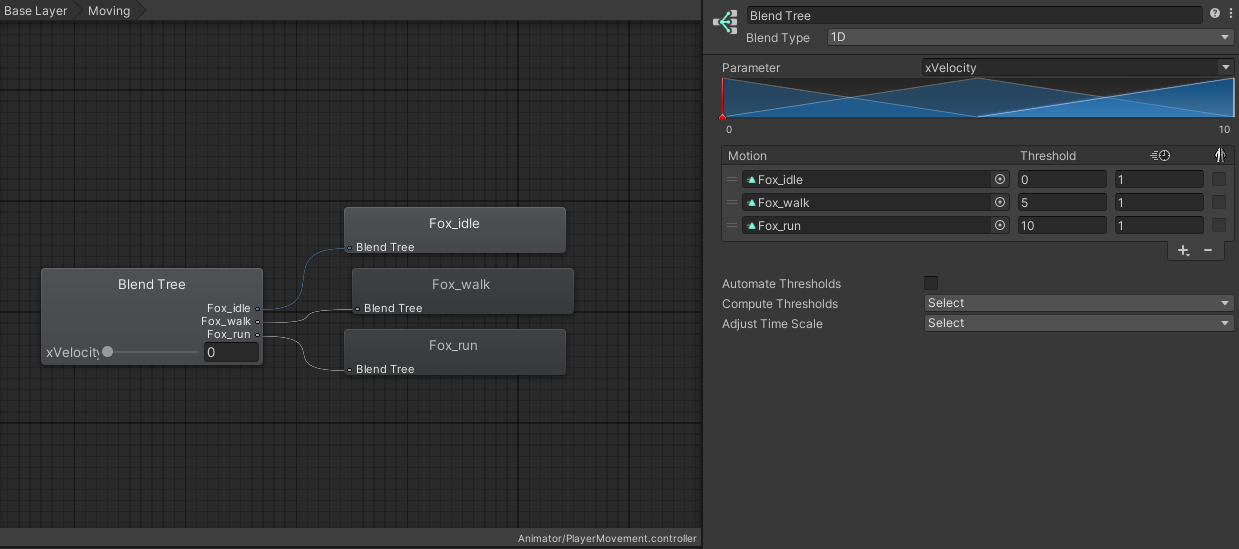
\includegraphics[scale = 0.45]{images/blendtree.png}
\caption{A Moving Blend Tree}
\label{fig:blendtree}
\end{figure}

A \aref{fig:blendtree}. ábrán látható, hogy a \texttt{Blend Tree} leginkább egy fa gráfra hasonlít. A különböző animációk küszöbértékei a jobb oldalon láthatóak. Ha az \texttt{xVelocity} értéke 0, akkor az \texttt{Fox\_idle} animáció játszódik le, ha az értéke 5, akkor a \texttt{Fox\_walk}, ha 10, akkor pedig a \texttt{Fox\_run}. Programból a paraméterek értékadása az \texttt{anim.SetBool;} és az \texttt{anim.SetFloat;} függvényekkel történnek. Ezeknek a függvényeknek a paraméterei az animátorban beállított paraméter neve és értéke.

\Section{A szintek elkészítése}

A következő lépésnek a szintek és a környezet megalkotását gondoltam, hiszen az elkészített animációkat itt lehet igazán kipróbálni és finomhangolni. Magát a pályát a Rule Tiles és a Tile Palette segítségével tudtam könnyedén elkészíteni. A Rule Tiles olyan C\# nyelven írt szkriptelhető tile-ok, amelyek elég okosak ahhoz, hogy a megfelelő szomszédos tile-okat használják, és menet közben kezelik a tile-ok animációját, a határokat és az ütközéseket. A Tile Palette pedig a Unity egyik beépített Tilemap készítő egysége. Ezután a hátteret készítettem el, amely követni fogja a kamera mozgását.

\SubSection{A Grib objektum, valamint a Tile Palette használata}

A Grid objektum a Tilemaps szülője vagy tárolója. Meghatározza a cellák elrendezését és a benne elhelyezett tile-ok szerkezetét. A Unityben a Grid komponens megszervezi a teret, amelyben a tile-ok elhelyezésre kerülnek, biztosítva, hogy azok egy meghatározott rácsrendszer szerint helyesen igazodjanak egymáshoz. \cite{unitytilemap}

A Tilemap egy olyan komponens, amely egy rácson belül működik, és a tile-ok gyűjteményét tárolja és kezeli. Lehetővé teszi a 2D tile alapú szintek gyors elkészítését a Tile Palette-ben meghatározott tile-ok felhasználásával.\cite{unitytilemap}

A Unity Tile Palette egy olyan eszköz, amellyel létrehozhatjuk, rendszerezhetjük és szerkeszthetjük a tile gyűjteményünket. A Tile Palette-et úgy tudjuk megnyitni, hogy a Windows fül 2D opciójánál kiválasztjuk azt. Ezután be kell importálni azokat az asset-eket, amelyekkel a pályát fogjuk elkészíteni, ekkor készítünk egy palettát melyet én külön mappába mentettem el. A blokkokat egyszerűen ki kell választani a palettából, és már el is tudjuk készíteni a pályánkat. Persze vigyázni kell, hogy a megfelelő blokkot válasszuk ki, különben esztétikailag nem lesz a legszebb a pályánk.  A TilePalette \aref{fig:tilepalette}. ábrán megtekinthető.

\begin{figure}[ht]
\centering
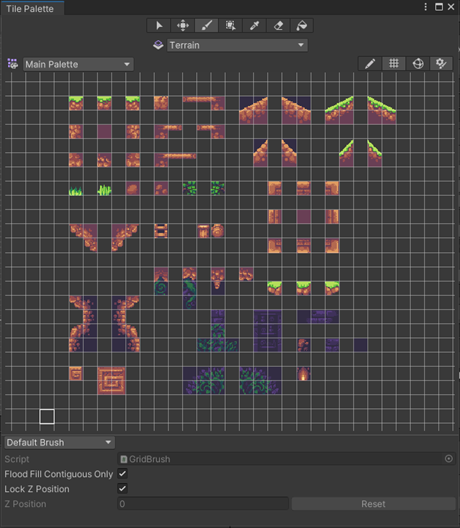
\includegraphics[scale = 0.8]{images/tilepalette.png}
\caption{A TilePalette}
\label{fig:tilepalette}
\end{figure}

Ezzel a palettával a Terrain nevű Tilemap-re fogok festeni. Fontos tudni, hogy ha több Tilemap-et hoz létre az ember, akkor mindenképpen válassza ki a megfelelőt, mielőtt nekiáll elkészíteni a pályát. Ennek a palettának a neve a Main Palette, ezen találhatóak azok a sprite-ok, amelyekkel a pályát készítettem el. Miután elkészítettem a pályát, a Terrain objektumhoz hozzá kellett adnom egy úgynevezett Tilemap Collider-t, ezután a rétegbeli sorrendjét kevesebbre kellett állítanom a Tilemap Renderer komponensnél, mint a Fox objektumét, különben eltakarta volna a karaktert. Az elkészített pályára elhelyeztem pár darab dekorációt, amelyek hangulatosabbá tették azt. Ezeket a dekorációkat a Props objektumban helyeztem el a rendszertelenség elkerülése végett.

Az első szint \aref{fig:firstlevel}. ábrán látható.

\begin{figure}[ht]
\centering
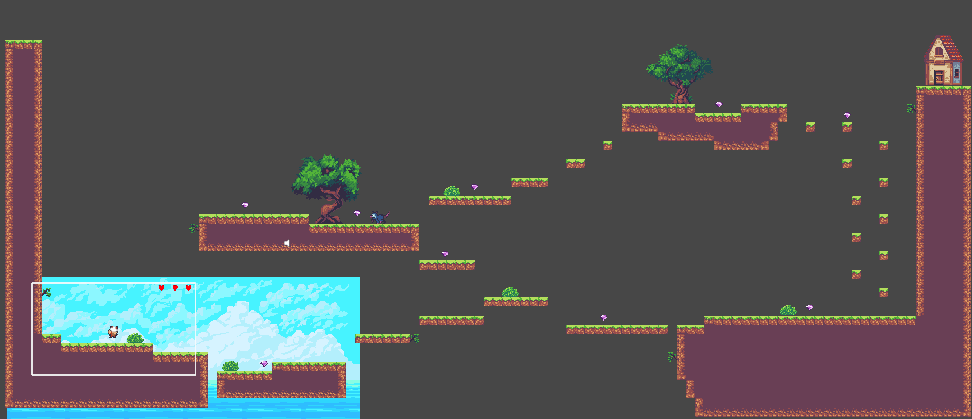
\includegraphics[width=\linewidth]{images/firstlevel.png}
\caption{A játékom első szintje}
\label{fig:firstlevel}
\end{figure}

\newpage
\SubSection{A RuleTiles használata}

Az első szintet még a RuleTiles használata nélkül készítettem el. Sajnos elég monoton és nehézkes volt az elkészítése, mert mindig oda kellett figyelni, hogy a megfelelő tile-t használjam. Ezért keresgélni kezdtem az interneten, hogy hogyan is lehetne a pályák elkészítését könnyebbé tenni, és ekkor bukkantam rá a RuleTiles-ra. A Rule Tile Asset egy hatékony és adaptív módja annak, hogy tile-okat fessünk egy jelenetbe. Általában a Tilemap használatakor a tile-ok festése viszonylag gyors, de ismétlődő és nehézkes is lehet, különösen, ha változtatásokat kell végrehajtani a tile-okon. A Rule Tiles ezzel szemben képes illeszkedni és alkalmazkodni a környező tile-okhoz, így gyors és kényelmes módját kínálja a tile-ok hozzáadásának vagy módosításának. Ha például egy Rule Tile-t festünk a Scene képernyőre a meglévő tile-ok mellé, a meglévő tile-ok automatikusan frissülnek. \cite{unityruletile}

Ahhoz, hogy létrehozzunk egy ilyen RuleTile-t, a fenti legördülő Assets menüpontból ki kell választanunk a Create fült, onnan a 2D-t, utána Tile-t és itt pedig a RuleTile-t amelyet én a Tiles mappába mentettem el Ground RuleTile néven. Ha kiválasztjuk, láthatjuk a tulajdonságait az Inspector fül alatt. Ha ezzel megvagyunk, készítenünk kell egy új palettát, és oda csak szimplán be kell húzni az elkészített RuleTile-t. Miután hozzáadtuk a palettánkhoz, ismét kiválasztjuk az általunk létrehozott RuleTile-t, és szabályokat kell hozzáadnunk. \cite{unityruletile} Én 9 szabályt adtam hozzá, a piros X az éleket jelöli, míg a zöld nyíl azt jelenti, hogy a tile folyamatos. A szabályok \aref{fig:ruletilerules}. ábrán láthatóak.

\begin{figure}[ht]
\centering
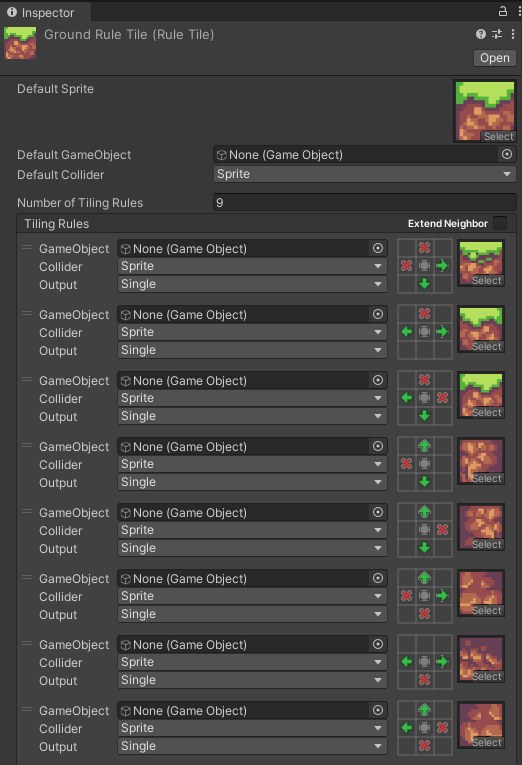
\includegraphics[scale = 0.5]{images/ruletilerules.png}
\caption{A RuleTile-om szabályai}
\label{fig:ruletilerules}
\end{figure}

\newpage
A szabályok beállítása után már kezdhetjük is a szintek könnyed és gyors elkészítését. \cite{unityruletile} A RuleTile segítségével elkészített alakzatok \aref{fig:ruletileshapes}. ábrán láthatóak.

\begin{figure}[ht]
\centering
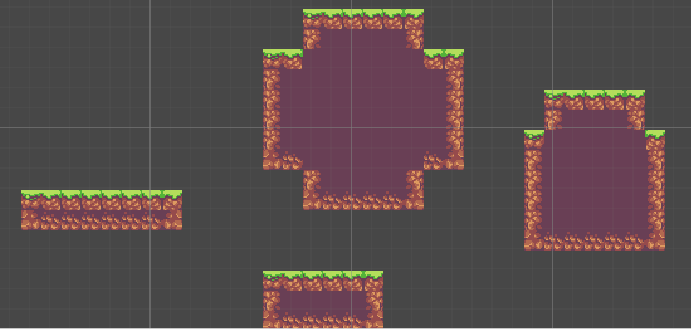
\includegraphics[scale = 0.5]{images/ruletileshapes.png}
\caption{A RuleTiles használatával elkészített példák}
\label{fig:ruletileshapes}
\end{figure}

\newpage
\Section{Interaktív elemek implementálása}

Az ellenség és a felvehető gyémántok animációját is az animator controller segítségével készítettem el. Egy féle ellenség van, egy oda-vissza mozgó oposszum. Az ellenségek száma a pálya szintjétől függ, minél magasabb a pálya szintje annál több ellenséget helyeztem el, így növelve a pálya nehézségét. A pályákat akkor teljesíti a játékos, ha kikerüli az ellenségeket, valamint felszedte az összes gyémántot. A gyémántok számát is növeltem a szintek nehezítése, és a hosszabb játékidő érdekében.

\SubSection{Az EnemyAI osztály}

Ezt az osztályt azért hoztam létre, hogy az ellenséges karaktert két meghatározott pont között oda-vissza mozgásra késztesse. A \texttt{[RequireComponent()]} attribútum a szkript elején arra szolgál, hogy egy BoxCollider2D komponens automatikusan hozzáadódjon minden olyan  GameObject-hez, amelyhez hozzácsatoljuk ezt a szkriptet. Készítettem egy \texttt{Reset()} metódust, amely akkor hívódik meg, amikor a szkriptet először adjuk hozzá egy GameObjecthez. Ez a metódus meghívja az \texttt{Init()} metódust, amely a kezdeti beállításokat konfigurálja. Ezek a beállítások a következők:
\begin{enumerate}
\item \texttt{BoxCollider2D} beállítása: A collider-t trigger módba állítja, hogy fizikailag ne blokkoljon más objektumokat, de mégis eseményeket váltson ki.
\item \texttt{Root} objektum létrehozása: Egy új „\texttt{\_Root}” nevű \texttt{GameObject} jön létre, amely az ellenség és annak útpontjai szülőjeként szolgál, így a hierarchia rendezett marad.
\item Útpontok beállítása: Két \texttt{waypoint} GameObject jön létre, és ezeknek a szülője, a Waypoints objektum, amely a Root gyereke. Ezek a pontok határozzák meg az ellenség „járőrútjának” a kezdő és végpontját.
\end{enumerate}

Ezt a szkriptet azért hoztam így létre, hogy ha újfajta ellenséget szeretnék a játékomba, akkor csak elég legyen hozzáadni az új ellenség objektumához. Az alábbi kódrészlet a \cite{youtubeplaylist} videósorozat alapján készült.

\begin{java}
private void Reset()
{
    Init();
}
void Init()
{
    //Make the BoxCollider isTrigger
    GetComponent<BoxCollider2D>().isTrigger = true;
    //Create root object
    GameObject root = new GameObject(name + "_Root");
    //Reset the position of root obj to enemy obj
    root.transform.position = transform.position;
    //Set enemy object as child of root
    transform.SetParent(root.transform);
    //Create Waypoints object
    GameObject waypoints = new GameObject("Waypoints");
    //Reset Waypoints position to root
    //Make Waypoints object child of root
    waypoints.transform.SetParent(root.transform);
    waypoints.transform.position =
        root.transform.position;
    //Create two points ( gameObject )
    //and reset their position to Waypoints object
    //Make the points children of Waypoints object
    GameObject p1 = new GameObject("Point1"); 
    p1.transform.SetParent(waypoints.transform);
    p1.transform.position = root.transform.position;
    GameObject p2 = new GameObject("Point2"); 
    p2.transform.SetParent(waypoints.transform);
    p2.transform.position = root.transform.position;

    //Init points list then add the points to it
    points = new List<Transform>();
    points.Add(p1.transform);
    points.Add(p2.transform);
}
\end{java}

Létrehoztam egy \texttt{Transform} típusú \texttt{points} nevű listát, amely azokat az útvonalakat jelöli, amelyek között az ellenség mozog. A \texttt{nextID} a következő útpont indexe a listában, amely felé az ellenség mozogni fog. Az \texttt{idChangeValue} egy olyan érték, amely vagy növeli, vagy csökkenti a \texttt{nextID}-t, meghatározva a következő útpont célpontját. A \texttt{speed} változó pedig az ellenség sebességét szabályozza.

Az \texttt{Update()} metódus a \texttt{MoveToNextLocation()} metódust hívja meg minden képkockafrissítésnél, hogy a mozgást lekezelje. A \texttt{MoveToNextLocation()} metódusban először meghatározzuk az aktuális cél útpontot. Ezután az ellenség orientációját fogjuk megvizsgálni, amely megfordítja az ellenség skáláját a következő pont iránya alapján, hogy arra fele nézzen amelyik útpont irányába halad. A \texttt{Vector2.MoveTowards()} funkciót használom az ellenségnek az aktuális pont felé történő mozgatására a meghatározott sebességgel. Ezután elvégzek egy közelség ellenőrzés (proximity check), ami annyit jelent, hogy amint az ellenség elég közel kerül az útponthoz (kevesebb, mint 1 egységnyi távolságra), ellenőrzöm, hogy melyik útpont felé haladjon tovább:
\begin{itemize}
\item Ha az utolsó pontnál járunk \texttt{(nextID == points.Count-1)}, akkor irányt váltunk az \texttt{idChangeValue} -1-re állításával.
\item Ha az első pontnál járunk \texttt{(nextID == 0)}, akkor az \texttt{idChangeValue} 1-re történő beállításával irányt változtatunk.
\item Ezután frissítem a \texttt{nextID}-t, hogy a következő útpontot célozza meg.
\end{itemize}

A szkript végén végrehajtok egy ütközésérzékelést az \texttt{OnTriggerEnter2D} módszerrel. Ha az ellenség ütközik egy „Player” címkével ellátott GameObjecttel, akkor a Fox objektumon (mivel csak ez van ellátva „Player” tag-gel) életvesztést hajt végre a \texttt{FindObjectOfType<LifeCount>().LoseLife()} metódus meghívásával. Az alábbi kódrészlet a \cite{youtubeplaylist} videósorozat alapján készült.

\begin{java}
void MoveToNextLocation()
{
    //Get the next Point transform
    Transform goalPoint = points[nextID];
    //Flip the enemy transform
    //to look into the point's direction
    if(goalPoint.transform.position.x > 
        transform.position.x ) 
    {
        transform.localScale = new Vector3(-7, 7, 1);
    }
    else
    {
        transform.localScale = new Vector3(7, 7, 1);
    }
    //Move the enemy towards the goal point
    transform.position = 
        Vector2.MoveTowards(transform.position, 
        goalPoint.position, speed * Time.deltaTime);
    //Check the distance between enemy and goal point
    //to trigger next point

    if(Vector2.Distance(transform.position, 
        goalPoint.position) < 1f)
    {
        //Check if we're at the end of the line
        //(make the change to -1)

        if(nextID == points.Count - 1)
        {
            idChangeValue = -1;
        }
        //Check if we're at the start of the line
        //( make the change to 1)

        if(nextID == 0)
        {
            idChangeValue = 1;
        }
        //Apply change on the next ID
        nextID += idChangeValue;
    }
}

private void OnTriggerEnter2D(Collider2D collision)
{
    if(collision.tag == "Player")
    {
        FindObjectOfType<LifeCount>().LoseLife();
    }
}
\end{java}

\SubSection{A LifeCount osztály}

Ez az osztály egy olyan osztály, amely a játékos életeinek a kezelésére szolgál a játékban, vizuális megjelenítést is biztosít a felhasználói felület elemein keresztül és kezeli a játék állapotát, ha a játékos életet veszít el.

Két publikus változót hoztam létre, az egyik az egy \texttt{Image} típusú tömb, amelyek UI elemek, amik a játékos életeit reprezentálják a felhasználói felületen. A másik az pedig az \texttt{int} típusú \texttt{livesCount} nevű változó, amelynek segítségével meghatározhatjuk, hogy hány élete legyen a játékosnak. A \texttt{LoseLife()} metódusban csökkentük a \texttt{livesCount} értékét eggyel, valamint a \texttt{lives[livesCount].enabled = false} paranccsal letiltjuk a \texttt{livesCount} indexnek megfelelő képet a \texttt{lives} tömbben. Ez a művelet vizuálisan megjeleníti egy élet elvesztését azáltal, hogy az egyik élet ikonját elrejti a felhasználói felületről. Ha a \texttt{livesCount} eléri a nulla értéket, akkor a \texttt{PlayerMovement} osztályban definiált \texttt{Death()} metódus hívódik meg. Az alábbi kódrészlet a \cite{youtubeplaylist} videósorozat alapján készült.

\begin{java}
public class LifeCount : MonoBehaviour
{
    public Image[] lives;
    public int livesCount;

    public void LoseLife()
    {
        //Decrease the value of lives remaining
        livesCount--;
        //Hide one of the life images
        lives[livesCount].enabled = false;  
        //If we run out of lives, we lose the game
        if(livesCount == 0)
        {
            FindObjectOfType<PlayerMovement>().Death();
        }
    }
}
\end{java}

\SubSection{Az InteractionSystem és az Item szkript}

Az létrehozott InteractionSystem szkript a Fox objektum és a gyűjthető tárgyak (Diamond objektum) közötti interakciók kezelésére szolgál. Először is létrehoztam egy pár darab detektálási paramétert. Az első a \texttt{Transform} típusú \texttt{detectionPoint}, ez az a pont, ahonnan az észlelési terület kiindul. Ez a játékos karakterhez csatlakozik egy a Fox objektum gyermekobjektuma, az ItemInteraction GameObject által. A \texttt{float} típusú \texttt{detectionRadius} meghatározza a \texttt{detectionPoint} körüli sugarat, amelyen belül az objektumokkal interakciót lehet folytatni. A \texttt{LayerMask} típusú \texttt{detectionLayer} megadja, hogy az észlelőrendszer melyik réteget vegye figyelembe, lehetővé téve a rendszer számára, hogy csak a megfelelően megjelölt objektumokat észlelje.

Ezután létrehoztam egy \texttt{GameObject} típusú \texttt{detectedObject} nevű változót, amely az éppen detektált objektum referenciáját tárolja, majd létrehoztam egy listát, amely a felvett tárgyakról tart listát. Mivel a felvevésnek hangja is van, ezért létrehoztam egy \texttt{SoundManager} típusú \texttt{audioManager} változót, amely egy hivatkozás a hangkezelőre, amely a felvevés hangot játsza le.

Az \texttt{Awake()} metódusom inicializálja az \texttt{audioManager}-t az „Audio” címkével ellátott GameObject megkeresésével és a SoundManager komponensének elérésével. Ez biztosítja a hanghatások lejátszását. Az \texttt{Update()} metódus ellenőrzi, hogy egy objektum felismerhető-e (\texttt{if(DetectObject())}). Ha a játékos megnyomja az E betűt, amivel interakciót folytathat az objektummal, akkor végrehajtja az \texttt{Interact()} metódust az észlelt objektum \texttt{Item} scriptjéből, és lejátsza a tárgyfelvételkor történő hangot. Az alábbi kódrészlet a \cite{youtubeplaylist} videósorozat alapján készült.

\begin{java}
private void Awake()
{
    audioManager = 
        GameObject.FindGameObjectWithTag(
            "Audio").
            GetComponent<SoundManager>();
}

void Update()
{
    if (DetectObject())
    {
        if(InteractInput())
        {
            detectedObject.
                GetComponent<Item>().
                Interact();
            audioManager.
                PlaySFX(
                audioManager.itemPickup);
        }
    }
}
\end{java}

A \texttt{DetectObject()} metódus a \texttt{Physics2D.OverlapCircle} függvényt használja a \texttt{detectionPoint} körüli \texttt{detectionRadius}-on belüli ütközők ellenőrzésére. Ezeket az ütközőket a \texttt{detectionLayer} alapján szűri ki. Ha egy ütközőt észlel, a detektált objektumot az észlelt GameObject-re állítja, és \texttt{true}-t ad vissza. Ha nem észlelt objektumot, törli a \texttt{detectedObject} értéket, és \texttt{false} értéket ad vissza.

A \texttt{PickUpItem()} metódus hozzáadja a megadott tárgyat a pickedItems listához, így ténylegesen nyomon követi a játék során összegyűjtött összes tárgyat. Az alábbi kódrészlet a \cite{youtubeplaylist} videósorozat alapján készült.

\begin{java}
bool DetectObject()
{
    Collider2D obj = 
        Physics2D.OverlapCircle
        (detectionPoint.position,
        detectionRadius,detectionLayer);

    if (obj == null)
    {
        return false;
    }
    else
    {
        detectedObject = obj.gameObject;
        return true;
    }
   
}

public void PickUpItem(GameObject item)
{
    pickedItems.Add(item);
}
\end{java}

Az Item szkript a játékban lévő tárgyakkal való interakciók kezelésére szolgál, és a felvehető tárgyakhoz nyújt funkcionalitást. Létrehoztam egy \texttt{enum} típusú változót, amelynek három értéke van: a \texttt{NONE}, a \texttt{PickUp}, amellyel a felvehetőséget jelzem és az \texttt{Examine}, amellyel a megvizsgálhatóságot jelzem. A megvizsgálható tárgyak jelenleg nem szerepelnek a játékomban, de a későbbiekben szeretném ezeket is belerakni. A \texttt{public InteractionType type} változó az interakció típusát tárolja. A \texttt{Reset()} metódus akkor hívódik meg, ha először csatoljuk egy GameObject-hez az Item szkriptet, beállítja a \texttt{[RequireComponent(typeof(BoxCollider2D))]} által már felcsatolt Collider2D komponenst, hogy triggerként működjön, és hozzárendeli a GameObject-et egy adott réteghez a \texttt{gameObject.layer = 7} paranccsal.

Az \texttt{Interact()} metódus egy \texttt{switch} utasítást tartalmaz, az interakció típusától függően különböző műveletek kerülnek végrehajtásra:
\begin{enumerate}
\item \texttt{PickUp}: Hozzáadja az elemet az InteractionSystem által kezelt felvett elemek listájához, majd értesíti a LevelManager-t, hogy egy Diamond objektumot begyűjtöttek és ezután letiltja a GameObject-et.
\item \texttt{Examine}: Ez a rész még nincs definiálva a megvizsgálható tárgyak hiánya miatt.
\end{enumerate}

\newpage
Az alábbi kódrészlet a \cite{youtubeplaylist} videósorozat alapján készült.
\begin{java}
public void Interact()
{
    switch (type)
    {
        case InteractionType.PickUp:
            FindObjectOfType<InteractionSystem>().
                PickUpItem(gameObject);
            FindObjectOfType<LevelManager>().
                GemCollected();
            //Disable the picked up object
            gameObject.SetActive(false);
            break;
        case InteractionType.Examine:
            break;
        default:
            break;
    }
}
\end{java}

\Section{A LevelManager és a SoundManager osztály}

A LevelManager osztály a játékszint különböző aspektusait kezeli, beleértve a játékosok előrehaladásának nyomon követését, a szintváltások kezelését és a játékbeli események kezelését, például a drágakövek gyűjtését és a szint befejezését. Először is létrehoztam egy \texttt{Vector2} típusú \texttt{playerInitialPos} nevű vektorváltozót, amelyben a Fox objektum kezdeti pozícióját fogom eltárolni a \texttt{Start()} metódusban. A \texttt{[SerializeField] GameObject completionPanel} arra szolgál, hogy a szünet menü referenciáját tárolja el. Az \texttt{int} típusú \texttt{totalGems} nevű változó megszámolja a szinten lévő felvehető objektumok számát a \texttt{Start()} metódusban található \texttt{FindGameObjectWithTag().Length} függvény segítségével.

A \texttt{Restart()} metódus arra szolgál, hogy ha a játékos elveszti mind a 3 életerejét, akkor a \texttt{PlayerMovement} osztály \texttt{Death()} metódusa meghívja azt. 
Újratöltöm a Scene-t a \texttt{SceneManager.LoadScene(SceneManager.GetActiveScene().name)} függvény segítségével, majd a kezdeti pozícióra állítom a játékos helyzetét. Az alábbi kódrészlet a \cite{youtubeplaylist} videósorozat alapján készült.

\begin{java}
public void Restart()
{
    //1 - Restart the scene
    SceneManager.LoadScene(
        SceneManager.GetActiveScene().name);
    //2 - Reset player pos
    FindObjectOfType<PlayerMovement>().
        transform.position = playerInitialPos;
}
\end{java}

A \texttt{GemCollected()} metódus a \texttt{gemsCollected} számlálót minden alkalommal növeli, amikor egy felvehető objektummal interakcióba lépett a játékos. Amikor az összegyűjtött drágakövek száma megegyezik a szinten rendelkezésre álló drágakövek teljes számával (\texttt{totalGems}), aktiválja a szint befejezését jelző panelt. Az alábbi kódrészlet a \cite{youtubeplaylist} videósorozat alapján készült.

\begin{java}
public void GemCollected()
{
    gemsCollected++;
    if (gemsCollected >= totalGems)
    {
        completionPanel.SetActive(true);   
    }
}
\end{java}

Található még a szkripten két metódus, a \texttt{LoadMainMenu()} és a \texttt{LoadNextLevel()} amelyek a szint befejézést jelző panel gombjainak a metódusai. A \texttt{LoadMainMenu()}-vel értelemszerűen a főmenüt töltjük be, a \texttt{LoadNextLevel()} metódussal pedig a következő szintet. Az alábbi kódrészlet a \cite{youtubeplaylist} videósorozat alapján készült.

\begin{java}
public void LoadMainMenu()
{
    SceneManager.LoadScene("Main Menu");
}

public void LoadNextLevel()
{
    SceneManager.LoadScene(
        SceneManager.GetActiveScene().
        buildIndex + 1);
}
\end{java}

A \texttt{SoundManager} osztály kezeli az összes hanggal kapcsolatos funkciót a játékban, beleértve a háttérzenét és a hangeffekteket (SFX). Először is létre kellett hoznom audiókomponenseket, ezek a hangforrások és a hangklippek. Az egyik hangforrás a \texttt{musicSource}, amelyhez a háttérzene lejátszásához hozzárendeltem a Unity szerkesztőjében a \texttt{Music} objektumot, amelynek az egyik komponense az \texttt{Audio Source}. A másik hangforrás pedig az \texttt{sfxSource}, amelyhez a hanghatások lejátszása érdekében ugyan úgy jártam el, mint a \texttt{musicSource} esetében, csak az SFX objektumot rendeltem hozzá. A háttérzene és a hangeffektek szétválasztása lehetővé teszi ezek hangerejének és beállításainak független kezelését. Négy darab hangklippet hoztam létre: \texttt{background},\texttt{ jumping}, \texttt{landing} és \texttt{itemPickup}.

Az \texttt{Awake()} metódusban a singleton mintát használtam annak biztosítására, hogy az \texttt{AudioManager} objektum csak egy példánya létezzen a jelenetek között. Ez elengedhetetlen a folyamatos hanglejátszás (például a háttérzene) fenntartásához a szintek közötti átmentek során. Az alábbi kódrészlet a \cite{youtubeplaylist} videósorozat alapján készült.

\begin{java}
private void Awake()
{
    if (instance == null)
    {
        instance = this;
        DontDestroyOnLoad(gameObject);
    }
    else 
    {
        Destroy(gameObject);
    }
}
\end{java}

A \texttt{Start()} metódus beállítja és elindítja a háttérzenét, amint a játék elkezdődik. A háttérzenét a Unity szerkesztőjében loop módra kell állítani ahhoz, hogy ha egyszer végigmegy a háttérzene, akkor újrakezdődjön. A \texttt{PlaySFX()} metódus egy egyszeri hanghatás lejátszása az \texttt{sfxSource} használatával, amely lehetővé teszi bármely átadott \texttt{AudioClip} lejátszását. Ez a módszer más szkriptekből is meghívható, például én a \texttt{PlayerMovement} szkriptből hívtam meg az ugrás és a landolás hangeffektek lejátszásához, valamint az \texttt{InteractionSystem} szkriptből, amikor a játékos felvesz egy gyémántot az \texttt{itemPickup} hangeffekt lejátszásához. Az alábbi kódrészlet a \cite{youtubeplaylist} videósorozat alapján készült.

\begin{java}
private void Start()
{
    musicSource.clip = background;
    musicSource.Play();
}

public void PlaySFX(AudioClip clip)
{
    sfxSource.PlayOneShot(clip);
}
\end{java}

\Section{A felhasználói felület elkészítése}

Ebben a fejezetben a játékom fő-, opció-, szintválasztó-, szünet- és a szint teljesítésekor előugró menü elkészítéséről, a hozzájuk tartozó szkriptek megírásáról lesz szó.

\SubSection{A főmenü}

A Unity-nek a beépített \texttt{UI} elemeit használtam fel a Main Menu nevezetű Scene elkészítéséhez. Amikor készítünk egy \texttt{UI} elemet, akkor a Unity automatikusan kreál egy \texttt{EventSystem} nevű objektumot, amely az eseményeket kezeli, valamint készít neki egy \texttt{Canvas} nevezetű szülőt a hierarchiában, ami igazából egy vászon amire illeszkedni fognak a \texttt{UI} elemek. A \texttt{Panel} és a \texttt{Button UI} elemeket használtam fel a főmenüm elkészítéséhez. A \texttt{Panel} objektumból 2 darab található, az egyik a \texttt{BackGround}, amelynek a \texttt{Source Image}-ét a játékomban található background sprite-ra állítottam. A második panel az úgymond egy keret, hogy jobban látszódjanak a \texttt{Button} objektumok. Három gombot készítettem el, a \texttt{Play}, az \texttt{Options} és a \texttt{Quit} gombokat. Mindhárom gombnak egy képet állítottam be háttérnek, amelyeket a Unity Asset Store-on találtam. Ha rámegyünk bármelyik \texttt{Button} objektumra, akkor az Inspector ablaknál van egy olyan opció, hogy \texttt{OnClick()}. Igazából ez egy metódus, és itt tudjuk beállítani, hogy hogy viselkedjen a gomb, ha az ember rákattint. Az \texttt{OnClick()} opció \aref{fig:onclick}. ábrán látható.

\begin{figure}[ht]
\centering
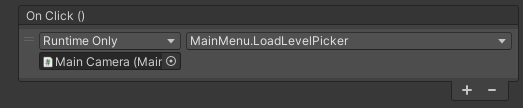
\includegraphics[scale = 0.9]{images/onclick.png}
\caption{A Button komponensen belüli OnClick() metódus}
\label{fig:onclick}
\end{figure}

Ehhez létrehoztam egy \texttt{MainMenu} szkriptet, amelyben létre kellett hoznom a megfelelő metódusokat, hogy mi történjen, ha mondjuk a játékos rákattint a Play, az Options vagy a Quit gombokra. Ez egy egyszerű szkript, amelyben három metódus található: a \texttt{LoadLevelPicker()}, a \texttt{LoadOptionsMenu()}, valamint a \texttt{QuitGame()}. A Unity-nek a \texttt{SceneManager} osztályát használtam fel arra, hogy a \texttt{LoadLevelPicker()} és a \texttt{LoadOptionsMenu()} metódusok betöltsék a megfelelő Scene-eket. Ezek a parancsok a \texttt{SceneManager.LoadSceneAsync(„Level Picker”)} a szintválasztó menühöz, és a opciók menühöz pedig a  \texttt{SceneManager.LoadSceneAsync(„Options Menu”)}. 
A \texttt{LoadScene()} funkcióval ellentétben, ez a funkció aszinkron módon tölti be az új jelenetet. A háttérben kezdi el a jelenet betöltését, lehetővé téve, hogy az aktuális jelenet tovább fusson, amíg az új jelenet készen nem áll. Ezzel kerülöm el a játék lefagyását a betöltés alatt. Ezt a szkriptet a \texttt{MainCamera} objektumhoz csatoltam, hogy a Button objektumok \texttt{OnClick()} metódusánál kiválasszam, és a megfelelő metódust rendeljem hozzá a gombokhoz. A Play gombhoz a \texttt{LoadLevelPicker()} metódust rendeltem, az Options gombhoz a \texttt{LoadOptionsMenu()} metódust, a Quit gombhoz pedig a \texttt{QuitGame()} metódust rendeltem hozzá. Az elkészült főmenü \aref{fig:mainmenu}. ábrán megtekinthető.

\begin{figure}[ht]
\centering
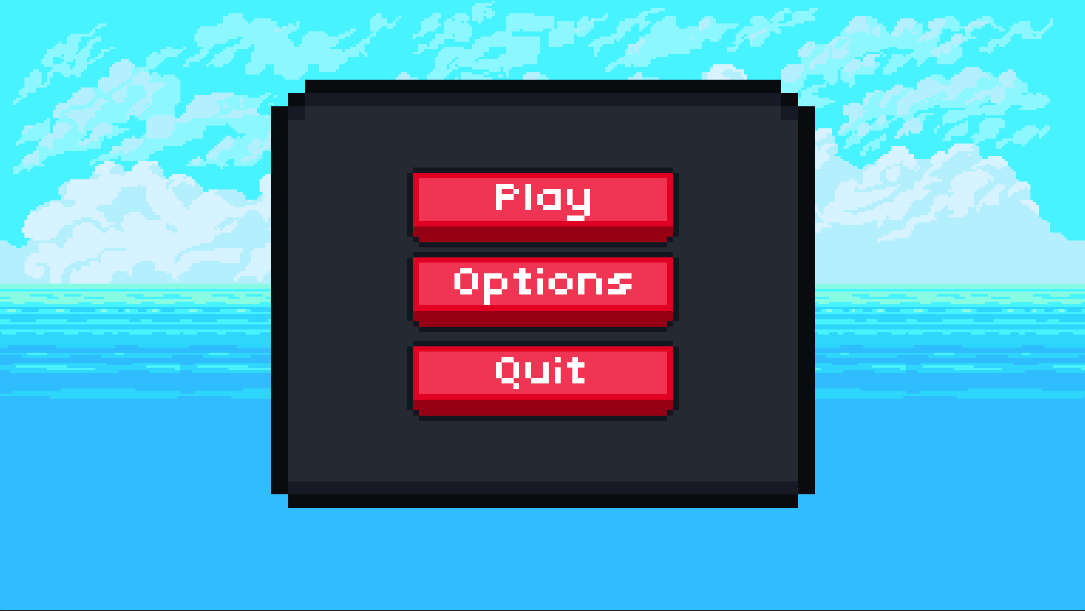
\includegraphics[scale = 0.4]{images/mainmenu.png}
\caption{A játék főmenüje}
\label{fig:mainmenu}
\end{figure}

\SubSection{A szint kiválasztásáért felelős menü}

A \texttt{Level Picker} menü elkészítésekor ugyan úgy jártam el, mint a főmenü elkészítésekor, annyi különbséggel, hogy itt nem három, hanem hét darab gombot helyeztem el a \texttt{Canvas} objektumon. Itt 5 darab gomb a játék szintjeinek a betöltéséért felelős, van egy vissza gomb, amely visszaviszi a játékost a főmenübe, valamint van egy \texttt{Dungeon} gomb is, amelynek segítségével a procedurális mapgeneráló algoritmus által kreált szint töltődik be. Ehhez írtam egy \texttt{LevelPicker} nevű szkriptet, amelynek a felépítése hasonlít a \texttt{MainMenu} szkript felépítéséhez. A szintválasztó menü \aref{fig:levelpicker}. ábrán megtekinthető.

\begin{figure}[ht]
\centering
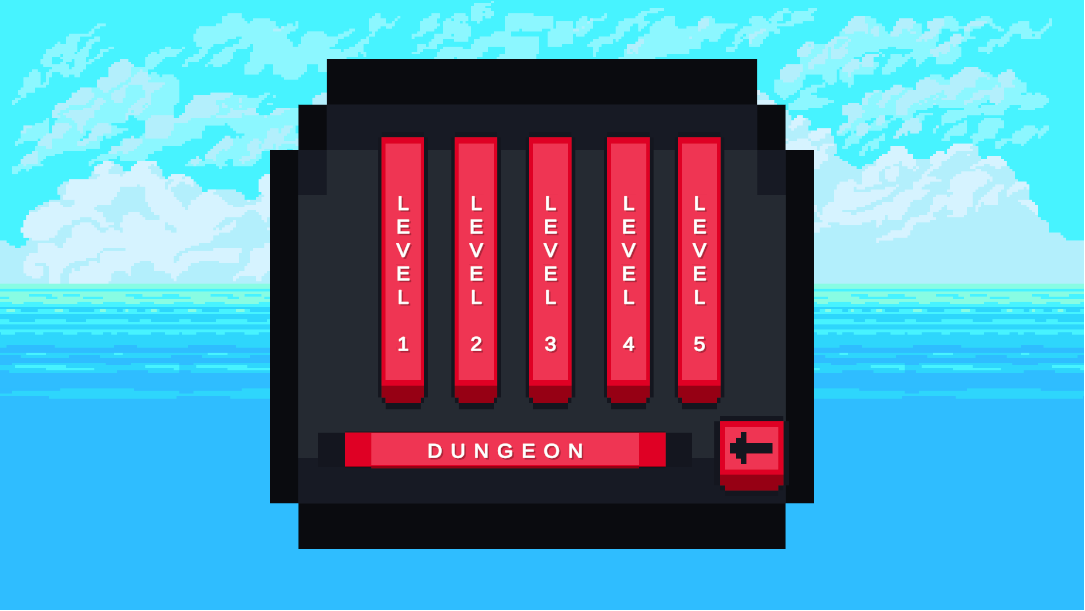
\includegraphics[scale = 0.4]{images/levelpicker.png}
\caption{A játékom \texttt{LevelPicker} menüje}
\label{fig:levelpicker}
\end{figure}

\SubSection{Az opciók menü}

Az opciók menü megalkotásánál a fő cél az az volt, hogy a játékban lévő háttérzene, valamint a hangeffektek hangerejét betudja állítani magának a játékos a saját tetszése szerint, valamint egy olyan gomb megalkotása, aminek a megnyomására a \texttt{Help} menü előjön. A hangerőszabályozáshoz a Unity beépített \texttt{Slider UI} elemét használtam. A \aref{fig:slider}. ábrán látható, hogy milyen \texttt{UI} elemekből épül is fel egy \texttt{Slider}. A \texttt{Background} elem az magának a \texttt{Slider}-nek a háttere, vagyis amikor teljesen levesszük a hangerőt, milyen színű legyen a csúszka, én ezt fehérre állítottam. A \texttt{Fill Area} gyermekobjektumát, a \texttt{Fill} objektumot én piros-ra állítottam. Piros színű lesz a slider, ha teljesen felvesszük a hangerőt. A \texttt{Handle Slide Area} gyermekobjektumát, a \texttt{Handle} objektumot alapértelmezetten hagytam, csak a színét állítottam át pirosra. Használtam még \texttt{Text UI} elemet is, hogy meg tudja a játékos különböztetni, hogy melyik hangerőt állítja éppen.

\begin{figure}[ht]
\centering
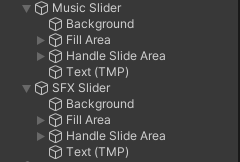
\includegraphics[scale = 1.0]{images/slider.png}
\caption{A Slider UI objektum}
\label{fig:slider}
\end{figure}

\newpage
Ahhoz, hogy a játékos tudja állítani a háttérzene és a hangeffektek hangerejét, készítenem kellett egy \texttt{AudioMixer}-t, valamint egy szkriptet. Az \texttt{AudioMixer} a Unity egyik nagy teljesítményű eszköze, amelyet a projektem hanganyagainak a kezelésére és keverésére használtam. Ez az eszköz lehetővé teszi a fejlesztők számára, hogy különböző hangforrások kezelésével és tulajdonságaik dinamikus beállításával szabályozzák a játékuk hangkörnyezetét. Én főleg a hangforrások csoportosításra használtam az \texttt{AudioMixer}-t, hogy kategorizáljam a háttérzene valamint a hangeffekteket. Az \texttt{AudioMixer}-ben, amely \aref{fig:audiomixer}. ábrán látható, 2 csoportot hoztam létre: a \texttt{Background} és az \texttt{SFX} csoportot, amelyeknek a Master a szülője. Ennek a két csoportnak a Volume változóját exponálnom / fel kellett tárnom a Unity szerkesztőjén belül ahhoz, hogy a \texttt{VolumeSettings} szkripten belül elérjem és manipulálhassam őket.

\begin{figure}
\centering
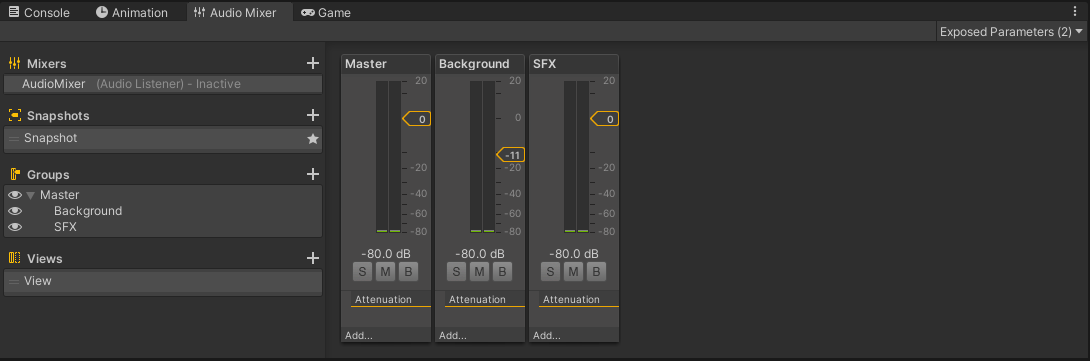
\includegraphics[width = \textwidth]{images/audiomixer.png}
\caption{Az \texttt{AudioMixer} eszköz}
\label{fig:audiomixer}
\end{figure}

A VolumeSettings szkriptben három \texttt{[SerializeField]}-el ellátott változót hoztam létre, az egyik az \texttt{AudioMixer} típusú \texttt{audioMixer} változó, amely a teljes hangkimenetet vezérli. Ezen a keverőn belül lévő speciális paraméterek (\texttt{music} és \texttt{SFXvolume}), amelyeket fel kellet tárnom a Unity szerkesztőjében, a hangerőszintek beállítására szolgálnak. A \texttt{Slider musicSlider} és a \texttt{Slider SFXSlider} a létrehozott Slider-ek referenciáit tárolják.

A \texttt{Start()} metódusban történnek az elmentett hangerőbeállítások betöltése vagy inicializálása. A szkript indításkor ellenőrzi, hogy vannak-e elmentett hangerőbeállítások (\texttt{PlayerPrefs.HasKey("musicVolume")}). Ha léteznek beállítások, akkor betölti azokat; ha nincsenek, akkor a hangerőszinteket az aktuális slider-ek pozíciója alapján állítja be. Ez biztosítja, hogy a hangerőre vonatkozó felhasználói beállítások a játékmenetek között is megmaradjanak. Az alábbi kódrészlet a \cite{volumesettings} videó alapján készült.

\begin{java}
private void Start()
{
    if (PlayerPrefs.HasKey("musicVolume"))
    {
        LoadVolume();
    }
    else 
    {
        SetBackgroundVolume();
        SetSFXVolume();
    }
}
\end{java}

A \texttt{SetBackgroundVolume()} és a \texttt{SetSFXVolume()} metódusok a hangerőszintek beállítására lettek létrehozva a megfelelő slider értékek alapján. A hangkeverő hangerőszintjét az \texttt{audioMixer.SetFloat} segítségével állítjuk be, ahol a hangerő értékét a \texttt{Mathf.Log10(volume) * 20} segítségével alakítjuk át. Ez a képlet a \texttt{slider} lineáris értékét logaritmikus skálára alakítja át, amely jobban utánozza az emberek hangszintérzékelését. Mindkét módszer elmenti az aktuális \texttt{slider}értékeket a \texttt{PlayerPrefs}-be, így a beállítások tartósak maradnak majd. Az alábbi kódrészlet a \cite{volumesettings} videó alapján készült.

\begin{java}
public void SetBackgroundVolume()
{
    float volume = musicSlider.value;
    audioMixer.SetFloat("music",
        Mathf.Log10(volume) * 20);
    PlayerPrefs.SetFloat("musicVolume", volume);
}

public void SetSFXVolume()
{
    float volume = SFXSlider.value;
    audioMixer.SetFloat("SFXvolume", 
        Mathf.Log10(volume) * 20);
    PlayerPrefs.SetFloat("SFXVolume", volume);
}
\end{java}

A \texttt{LoadVolume()} metódus a \texttt{PlayerPrefs}-ből lekérdezi a mentett hangerőbeállításokat, és ennek megfelelően frissíti a csúszkák pozícióit. Itt meghívásra kerülnek a \texttt{SetBackgroundVolume()} és a \texttt{SetSFXVolume()} metódusok, hogy a hangkeverő beállításai frissüljenek a betöltött értékeknek megfelelően.

Az elkészült szkriptet a Canvas objektumhoz csatoltam, majd ezt a Canvas objektumot a Slider objektumok Slider komponensénél lévő On Value Changed metódusnál referáltam, hogy a megfelelő funkciót ki tudjam választani a két csúszkának.

A következő lépés egy kisebb szkript írása, amely majd a vissza gomb és a Help gomb metódusait fogja tartalmazni. Ezt \texttt{OptionsMenu} nevén neveztem el, és ez a szkript három metódust tartalmaz. Az egyik, a \texttt{LoadMainMenu()} amely a vissza gomb metódusa, és betölti a játék főmenüjet, a másik a \texttt{LoadHelpMenu()}, amely a Canvas objektumban lévő HelpMenu objektumot hozza elő, valamint az OptionsMenu objektumot eltünteti. A harmadik metódus a \texttt{BackToOptions()}, amely eltüneti a HelpMenu objektumot, és előhozza az OptionsMenu objektumot. 
\newpage
Az OptionsMenu objektum \aref{fig:optionsmenu}. ábrán, a HelpMenu objektum \aref{fig:helpmenu}. ábrán tekinthető meg.

\begin{figure}[ht]
\centering
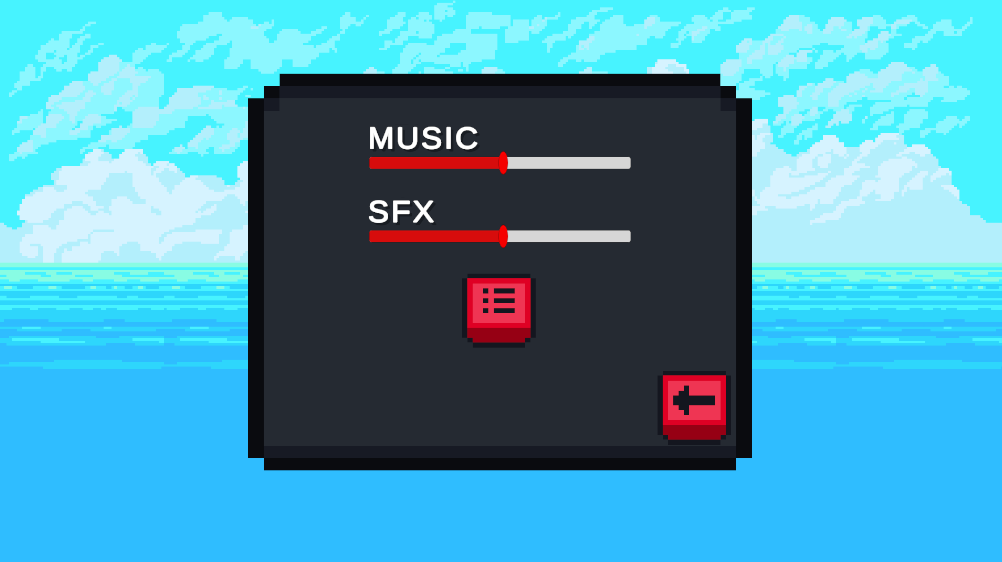
\includegraphics[width =0.9 \textwidth]{images/optionsmenu}
\caption{A játék opciók menüje}
\label{fig:optionsmenu}
\end{figure}

\begin{figure}[ht]
\centering
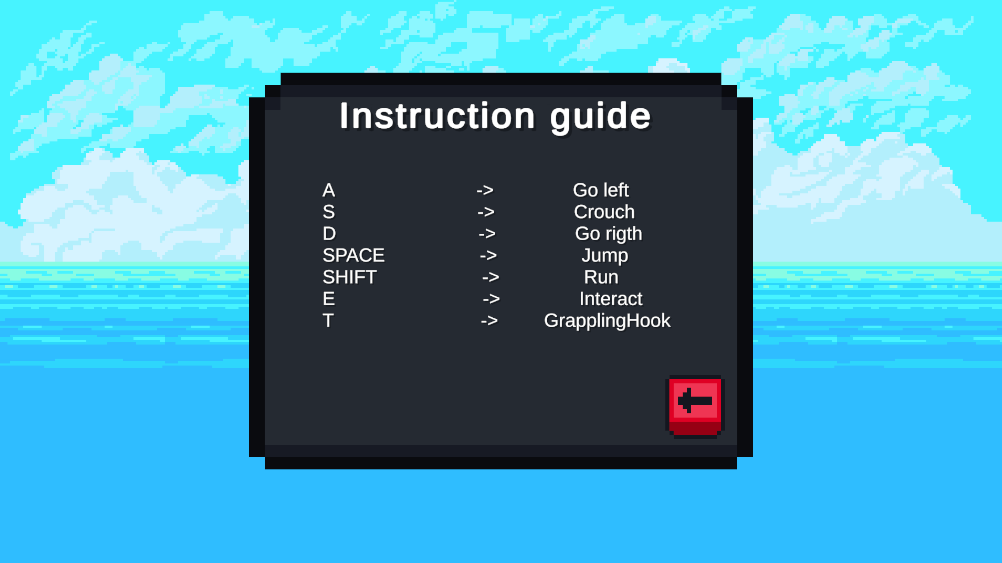
\includegraphics[width =0.9 \textwidth]{images/helpmenu}
\caption{A HelpMenu UI objektum}
\label{fig:helpmenu}
\end{figure}





